\titleformat{\chapter}[display]{\bfseries\centering}{\huge Chapter \thechapter}{1em}{\Huge #1}
\newgeometry{top=3cm, bottom=2.2cm, left=3cm, right=2cm, headsep=1.2cm, footskip=1cm, headheight=0.3cm, textheight=24.5cm, textwidth=16cm}
\onehalfspacing
\pagestyle{fancy}
\fancyhf{}
\renewcommand{\headrulewidth}{0pt}
\cfoot{\thepage}
\chapter{Proposed System}

\section{Detailed explanation of Proposed system}
\subsection{Block diagram of Proposed system / Workflow}
\begin{figure}[H]
\centering
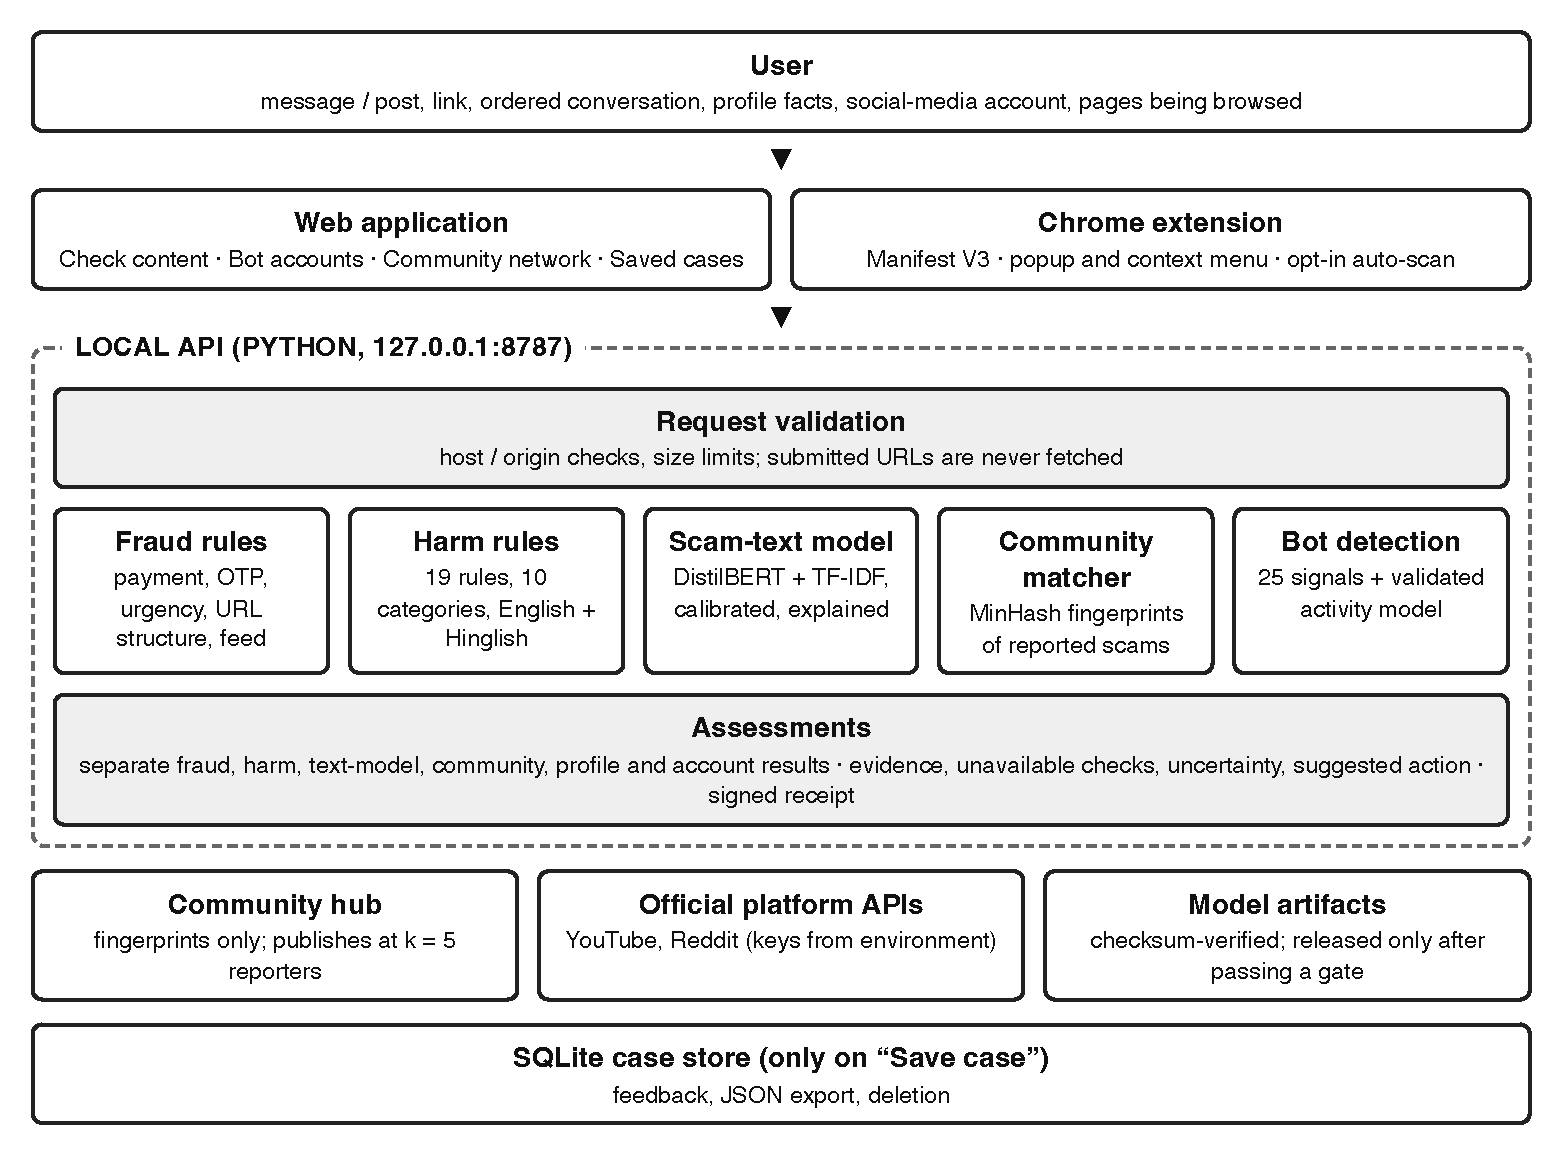
\includegraphics[width=0.86\linewidth]{dia2/block_v2.pdf}
\caption{Block Diagram of Proposed System / Workflow}
\label{fig:block}
\end{figure}
\begin{figure}[H]
\centering
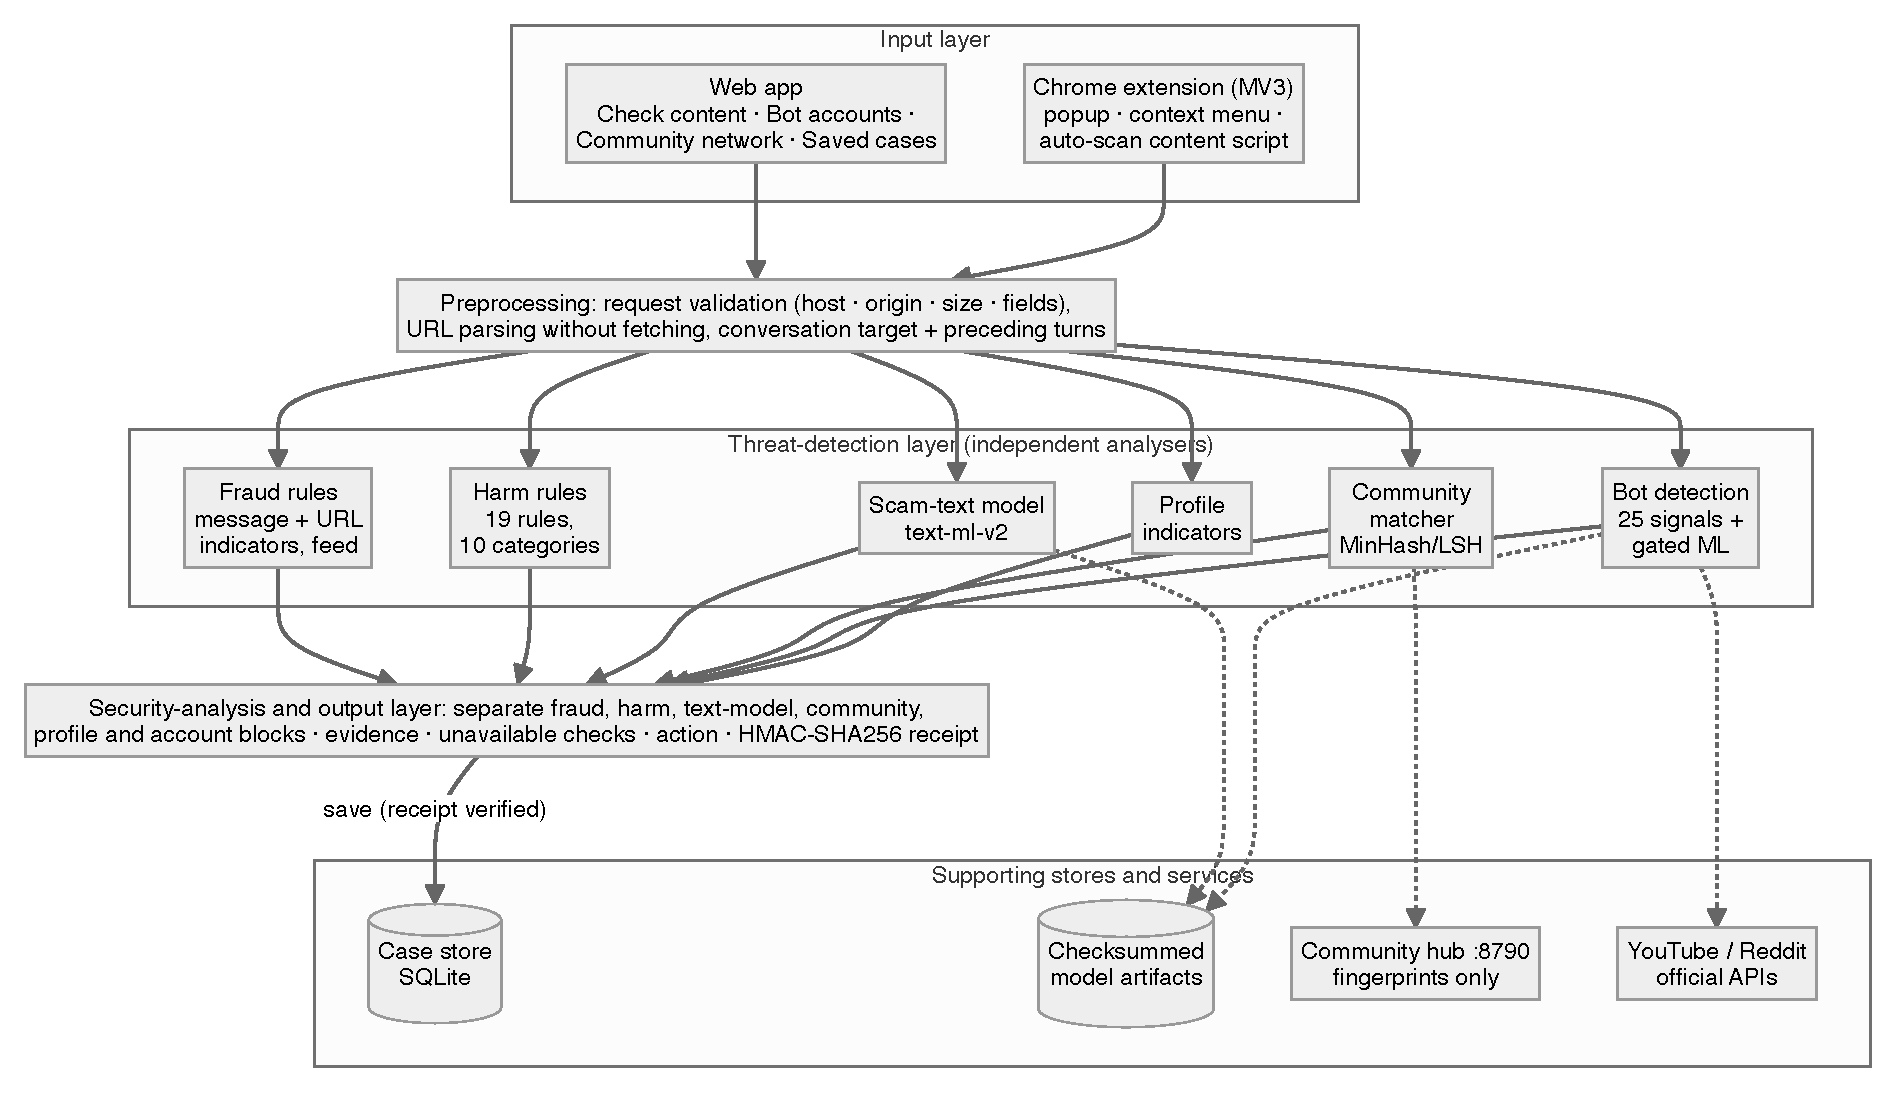
\includegraphics[width=0.92\linewidth]{dia2/arch_v2.pdf}
\caption{Layered Architecture of Sentinel}
\label{fig:arch}
\end{figure}

\subsection{Working Principle (Algorithm)}
\noindent Sentinel works as a local safety assistant. It receives what the user wants to check, runs several independent checkers on it, and shows each result with its reasons. The working of the system can be summarised as follows:
\begin{enumerate}
\item \textbf{Input Collection:} the user pastes a message, link, chat or account into the web app, uses the extension popup, or switches on auto-scan for a site.
\item \textbf{Request Validation:} the local server accepts requests only from the user's own computer and the extension, rejects empty or oversized requests, and never opens the submitted link.
\item \textbf{Fraud Rules:} the message is checked for requests for money, passwords or OTPs and for urgency; the link is checked for warning signs such as an IP address or punycode.
\item \textbf{Harm Rules:} the text is cleaned of disguises and checked by 19 rules for threats, self-harm, sextortion, harassment and other harmful language in English and Hinglish.
\item \textbf{Scam-Text Model:} a learned model estimates the probability that the message is a scam and highlights the words that raised the score.
\item \textbf{Community Matching:} the message's fingerprint is compared with scam campaigns reported by other users.
\item \textbf{Bot Detection:} for an account, 25 behaviour signals are scored and a trained model adds a probability where it is allowed.
\item \textbf{Result Assembly:} each checker returns its own level (High, Review or Low concern), its evidence, what it could not check and a next step. A signed receipt is attached.
\item \textbf{Display and Action:} the results are shown as cards or as markers on the page. The user can save the case, and can choose to share a scam's fingerprint with the community.
\item \textbf{Continuous Scanning:} with auto-scan on, steps 2--9 repeat as new messages appear on the page.
\end{enumerate}

\subsection{Phase / Module - wise explanation (as per workflow)}
\noindent Sentinel is divided into phases according to the workflow. Each phase performs one job and passes its output to the next.

\subsubsection*{Phase 1: Input Capture}
\noindent The \textbf{web app} has four pages: \emph{Check content}, \emph{Bot accounts}, \emph{Community network} and \emph{Saved cases}. The \textbf{Chrome extension} offers a popup, a right-click menu and \emph{auto-scan}. When auto-scan is on for a site, the extension reads the text visible on screen (and text or QR codes inside images, using on-device OCR) and sends it in small batches to the local server.\\
\textbf{Output:} a check request (message, link, chat, profile or account).

\subsubsection*{Phase 2: Request Validation}
\noindent The Python server listens only on the user's computer (127.0.0.1). It rejects requests from other websites, limits the request size, and adds browser security headers. Links are read as text and never visited.\\
\textbf{Output:} a clean, safe request.

\subsubsection*{Phase 3: Fraud Rules}
\noindent Rules look for requests for money or fees, passwords or OTPs, and urgency, and for link warning signs: an IP address instead of a name, ``@'' in the address, punycode, many sub-domains or a very long link. An optional list of known phishing links can be loaded.\\
\textbf{Output:} fraud level with evidence.

\subsubsection*{Phase 4: Harmful-Language Rules}
\noindent 19 rules in 10 groups cover threats, mass violence, self-harm, sextortion, blackmail, stalking, hate and harassment, in English and Hinglish. The text is first cleaned (\texttt{1d10t}$\to$idiot, \texttt{k.y.s}$\to$kys, \texttt{stuuupid}$\to$stupid). Idioms such as ``this movie killed it'' are ignored, ``I would never hurt you'' is not a threat, and quoted insults go to human review. Self-harm messages get helpline numbers (Tele-MANAS 14416) \cite{telemanas}.\\
\textbf{Output:} harm level, categories and advice.

\subsubsection*{Phase 5: Scam-Text Model}
\noindent A DistilBERT model and a TF-IDF model are averaged to label a message as genuine, spam or smishing. The probability is calibrated, and a warning is given at 61.1\% or more. The words that raised the score are highlighted.\\
\textbf{Output:} scam probability and key words.

\subsubsection*{Phase 6: Community Network}
\noindent When a scam is found, Sentinel can (if the user agrees) send only a \emph{fingerprint} of it to a hub. When 5 different users report the same scam, the hub publishes it, and every user is warned, even if their own model missed it. The hub never sees the message text.\\
\textbf{Output:} match with a known scam campaign, if any.

\subsubsection*{Phase 7: Bot Detection}
\noindent An account is checked using data from the official YouTube or Reddit APIs, an uploaded file or typed details; profiles are never scraped. 25 signals such as posting rhythm, repeated posts and follower ratio are scored, and the signals that mattered are shown. A trained activity model adds a probability for X accounts.\\
\textbf{Output:} bot score, confidence and top signals.

\subsubsection*{Phase 8: Result Assembly and Storage}
\noindent The results are kept separate and each carries evidence, missing checks and a next step. A signed receipt (HMAC) is attached, so a case can be saved only exactly as the user saw it. Saved cases are kept in a local SQLite file and can be exported or deleted.\\
\textbf{Output:} result cards, page markers and optional saved case.

\section{System Analysis}
\subsection{Functional Requirements}
\noindent Functional requirements describe the services that Sentinel must provide:
\begin{enumerate}
\item \textbf{Content Input:} the system shall accept a message, link, chat, profile details or account, alone or together.
\item \textbf{Input Validation:} the system shall reject empty, oversized or invalid requests with a clear error.
\item \textbf{Safe Link Handling:} the system shall never open a submitted link or scrape a profile.
\item \textbf{Fraud Check:} the system shall detect money, OTP and urgency requests and suspicious link patterns.
\item \textbf{Harmful-Language Check:} the system shall detect harmful language in English and Hinglish and give advice by urgency.
\item \textbf{Scam-Text Model:} the system shall give a calibrated scam probability and the words behind it.
\item \textbf{Auto-Scan:} the system shall scan visible page text only on sites the user switched on, and mark risky items.
\item \textbf{Community Sharing:} the system shall share only anonymous fingerprints with the hub, and only if the user agrees.
\item \textbf{Account Check:} the system shall analyse accounts from official APIs, uploads or manual entry, and reject unsafe profile links.
\item \textbf{Separate Results:} the system shall report each threat separately, with evidence, missing checks and an action.
\item \textbf{Case Management:} the system shall save, list, export and delete cases, and save only with a valid receipt.
\end{enumerate}

\subsection{Non-Functional Requirements}
\begin{enumerate}
\item \textbf{Privacy:} everything runs on the user's computer; nothing is stored unless saved; the hub stores no message text.
\item \textbf{Security:} local-only server, origin checks, size limits, security headers, signed receipts, rate limits, and API keys only from environment variables.
\item \textbf{Explainability:} every result explains its evidence in plain words.
\item \textbf{Real-Time Performance:} rule checks take milliseconds and the text model about 2 ms per message on a laptop CPU.
\item \textbf{Reliability:} a broken model or offline hub shows ``unavailable'' and never breaks the check.
\item \textbf{Usability:} results are shown as simple cards with a clear next step.
\item \textbf{Compatibility:} runs on Windows, macOS or Linux with Python and Google Chrome.
\end{enumerate}

\subsection{Specific Requirements}
\subsubsection*{Input Requirements}
\begin{itemize}
\item \textbf{Message Input:} the text of a message or post, up to 4,000 characters per scanned item.
\item \textbf{Link Input:} a URL of up to 2,048 characters, read as text only.
\item \textbf{Conversation Input:} ordered chat turns with one selected target message.
\item \textbf{Account Input:} a YouTube, Reddit or X profile link, or a JSON/CSV file of the account's posts.
\end{itemize}

\subsection{Software and Hardware Requirements}
\subsubsection*{Software Requirements}
\begin{itemize}
\item \textbf{Operating System:} Windows 10/11, macOS or Linux.
\item \textbf{Programming Languages:} Python for the server and models; JavaScript, HTML and CSS for the web app and extension.
\item \textbf{Machine Learning:} PyTorch and Transformers for training; ONNX Runtime and scikit-learn for running the models.
\item \textbf{Database:} SQLite (built into Python).
\item \textbf{Browser:} Google Chrome, with the Sentinel extension loaded.
\item \textbf{Testing and Version Control:} Python \texttt{unittest}, Node.js test runner, Git and GitHub.
\end{itemize}
\subsubsection*{Hardware Requirements}
\begin{itemize}
\item \textbf{Computer:} a laptop or desktop; Sentinel was developed and tested on laptops with 16 GiB RAM (AMD Ryzen 7 7435HS and Apple M4).
\item \textbf{Storage:} space for model files and datasets.
\item \textbf{Network:} not needed for checks; only for the optional YouTube/Reddit APIs and dataset downloads.
\end{itemize}

\subsection{Use Case Modelling}
\noindent Use case modelling describes how the actors interact with Sentinel. The three major use cases are:
\begin{enumerate}
\item Check Content
\item Auto-Scan a Page
\item Check an Account
\end{enumerate}
\begin{figure}[H]
\centering
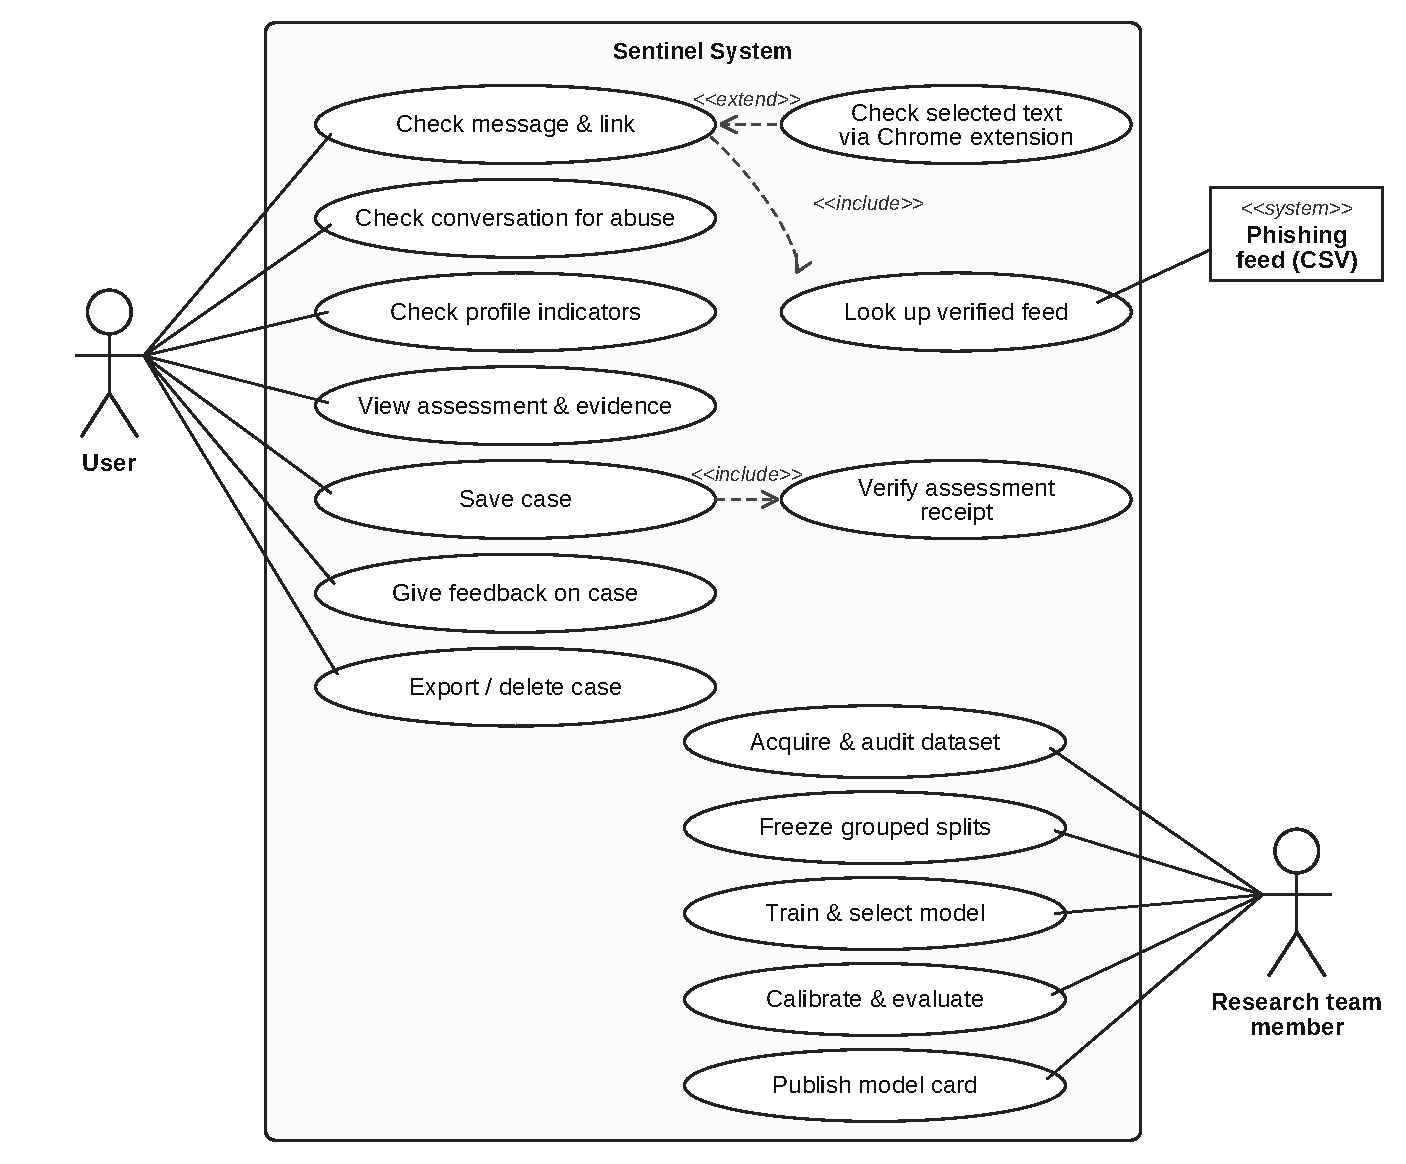
\includegraphics[width=0.8\linewidth]{dia/usecase.pdf}
\caption{Use Case Diagram of Sentinel}
\label{fig:usecase}
\end{figure}

\subsubsection*{UC-01: Check Content}
\noindent\textbf{Actor:} User\\
\textbf{Objective:} find out whether a message or link is a scam or harmful.\\
\textbf{Description:} the user pastes a message, link or chat into the web app or extension. Sentinel runs all checkers and shows a separate result for each threat.\\
\textbf{Main Flow:}
\begin{enumerate}
\item User pastes the content and clicks \emph{Analyze}.
\item The server validates the request.
\item Fraud rules, harm rules, the scam-text model and the community matcher run.
\item The results are assembled with a signed receipt.
\item Result cards with evidence and a next step are shown.
\end{enumerate}
\textbf{Output:} result cards; the user may save the case.

\subsubsection*{UC-02: Auto-Scan a Page}
\noindent\textbf{Actor:} User\\
\textbf{Objective:} be warned about risky messages while browsing.\\
\textbf{Description:} the user turns on auto-scan for a site. The extension reads visible text and images and marks risky items on the page.\\
\textbf{Main Flow:}
\begin{enumerate}
\item User switches on auto-scan for the site and allows access.
\item The extension collects visible text and new messages.
\item Batches are sent to the local server and checked.
\item Each item gets a severity: high, review or none.
\item Risky items are marked and counted on the toolbar badge.
\end{enumerate}
\textbf{Output:} markers on the page; the page itself is not changed.

\subsubsection*{UC-03: Check an Account}
\noindent\textbf{Actor:} User\\
\textbf{Objective:} find out whether an account behaves like a bot.\\
\textbf{Description:} the user enters a profile link or uploads the account's posts. Sentinel scores behaviour signals and shows which ones matter.\\
\textbf{Main Flow:}
\begin{enumerate}
\item User enters a link or uploads a file.
\item The link is checked against allowed platforms (never opened directly).
\item Data is fetched from the official API or read from the file.
\item 25 signals are scored and a trained model adds a probability where allowed.
\item If too little data is available, the score is not shown.
\end{enumerate}
\textbf{Output:} bot score, confidence and top signals.

\section{Proposed System: Analysis, Modelling and Design}
\subsection{UML Diagrams}
\noindent The following UML diagrams show the structure and working of Sentinel.
\begin{figure}[H]
\centering
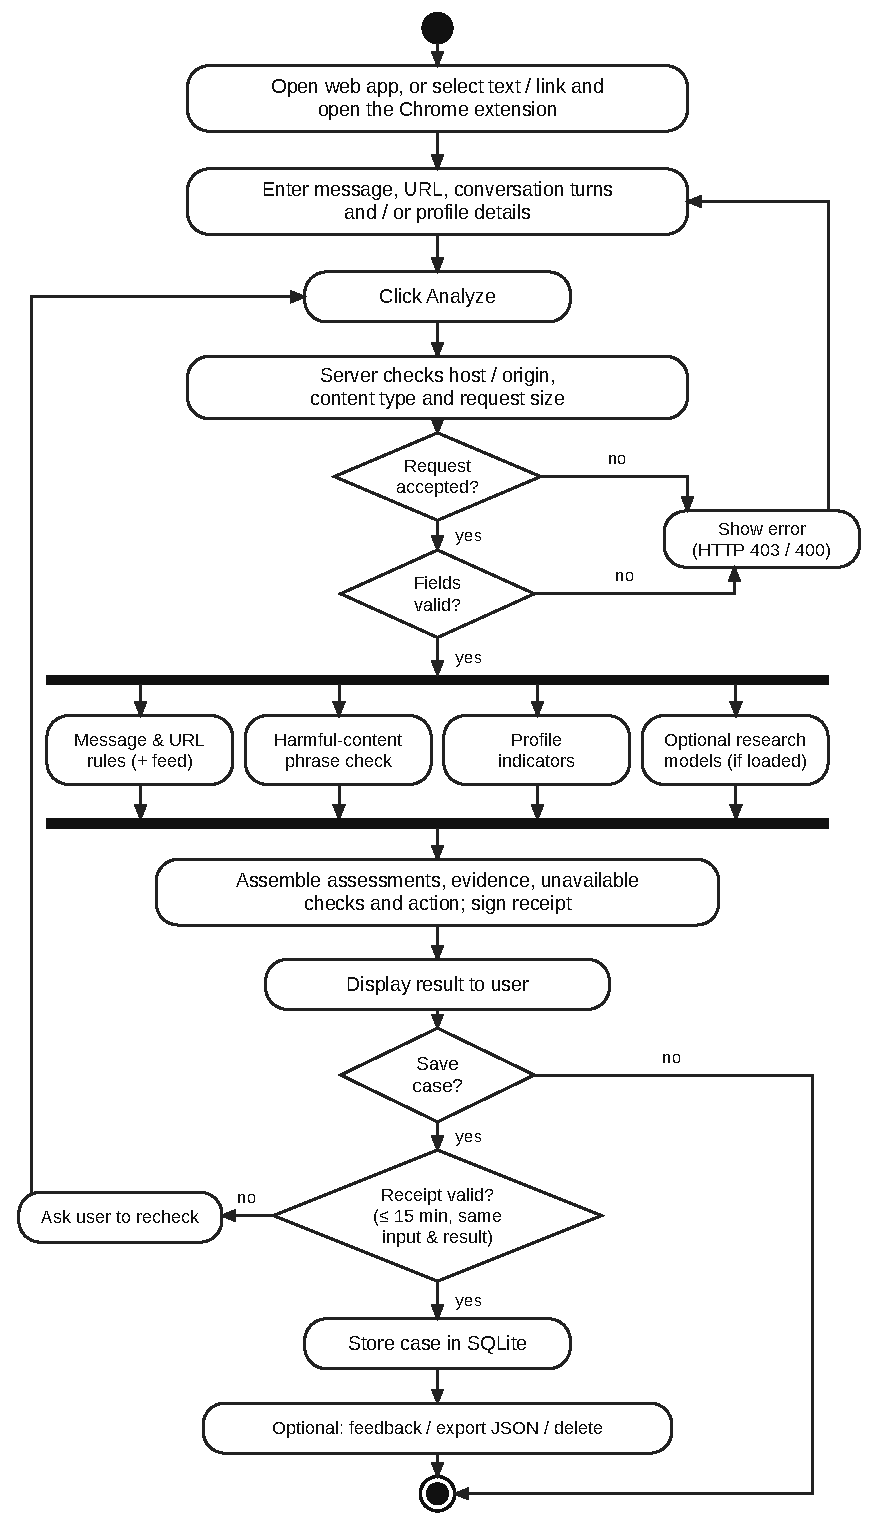
\includegraphics[height=0.55\textheight]{dia/activity.pdf}
\caption{Activity Diagram}
\label{fig:activity}
\end{figure}
\begin{figure}[H]
\centering
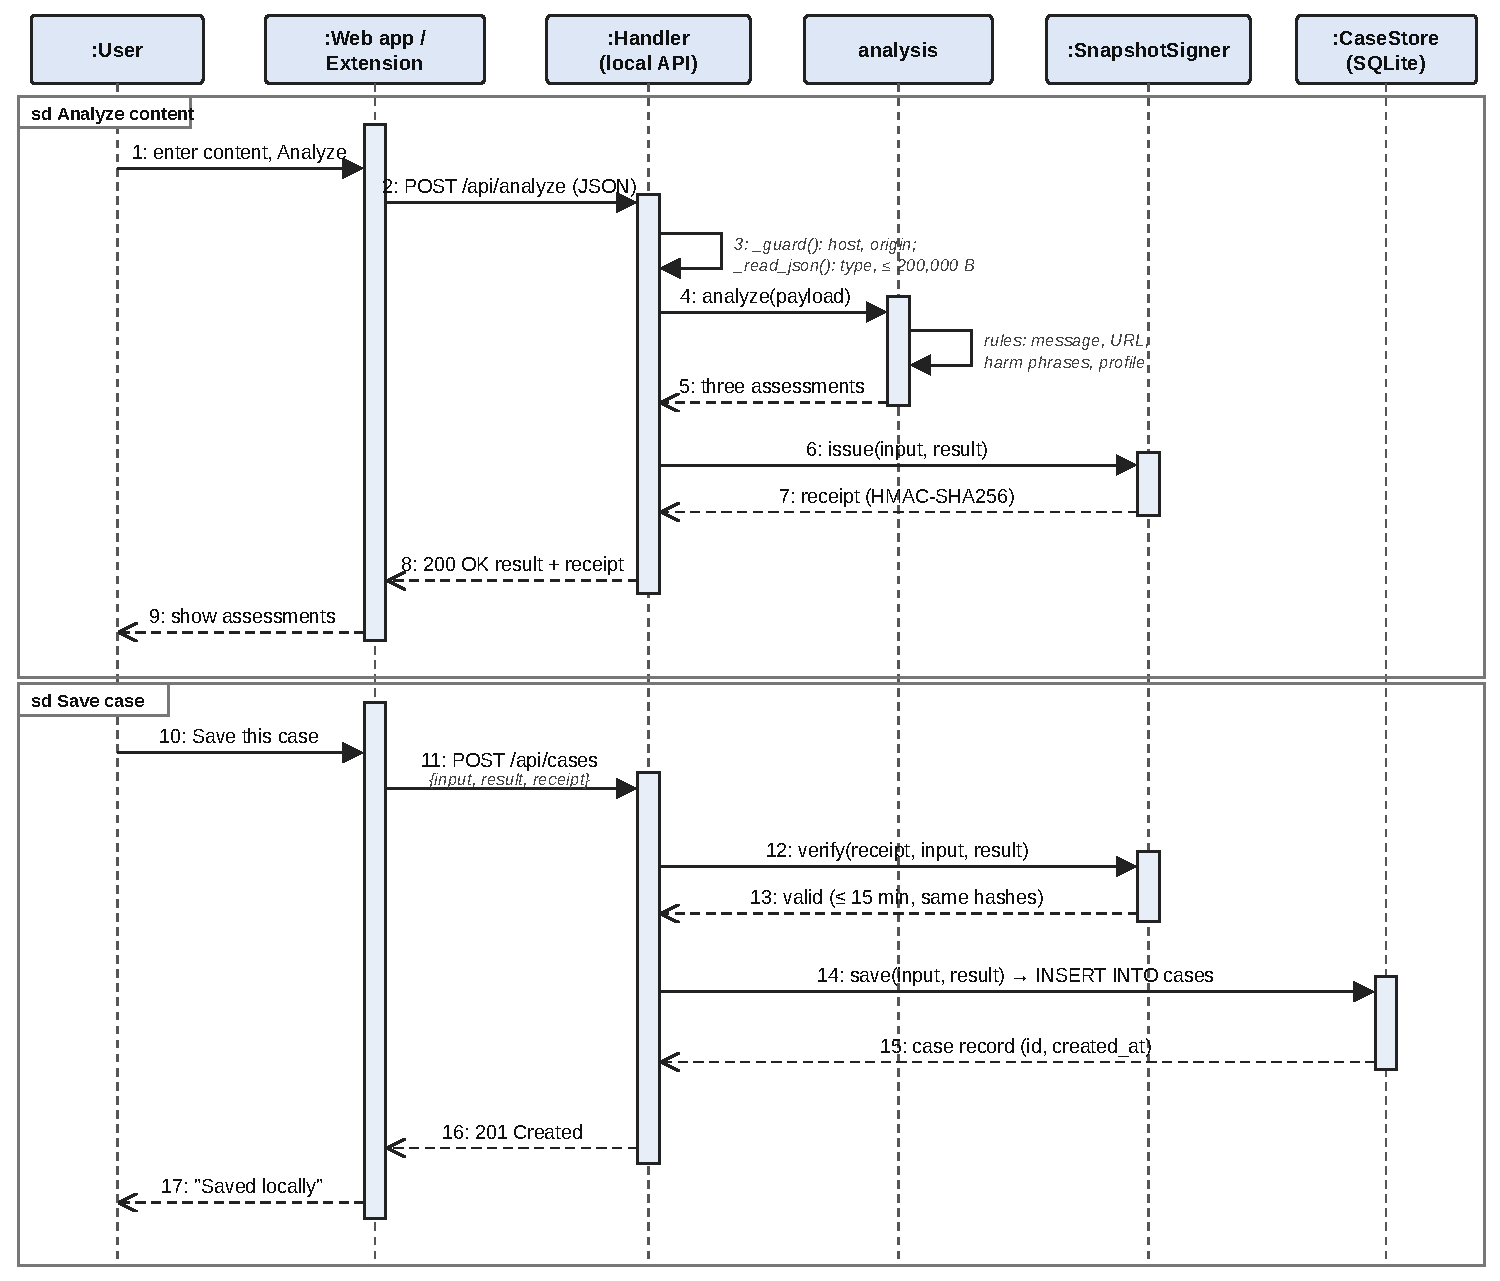
\includegraphics[width=\linewidth]{dia/sequence.pdf}
\caption{Sequence Diagram: Checking and Saving Content}
\label{fig:sequence}
\end{figure}
\begin{figure}[H]
\centering
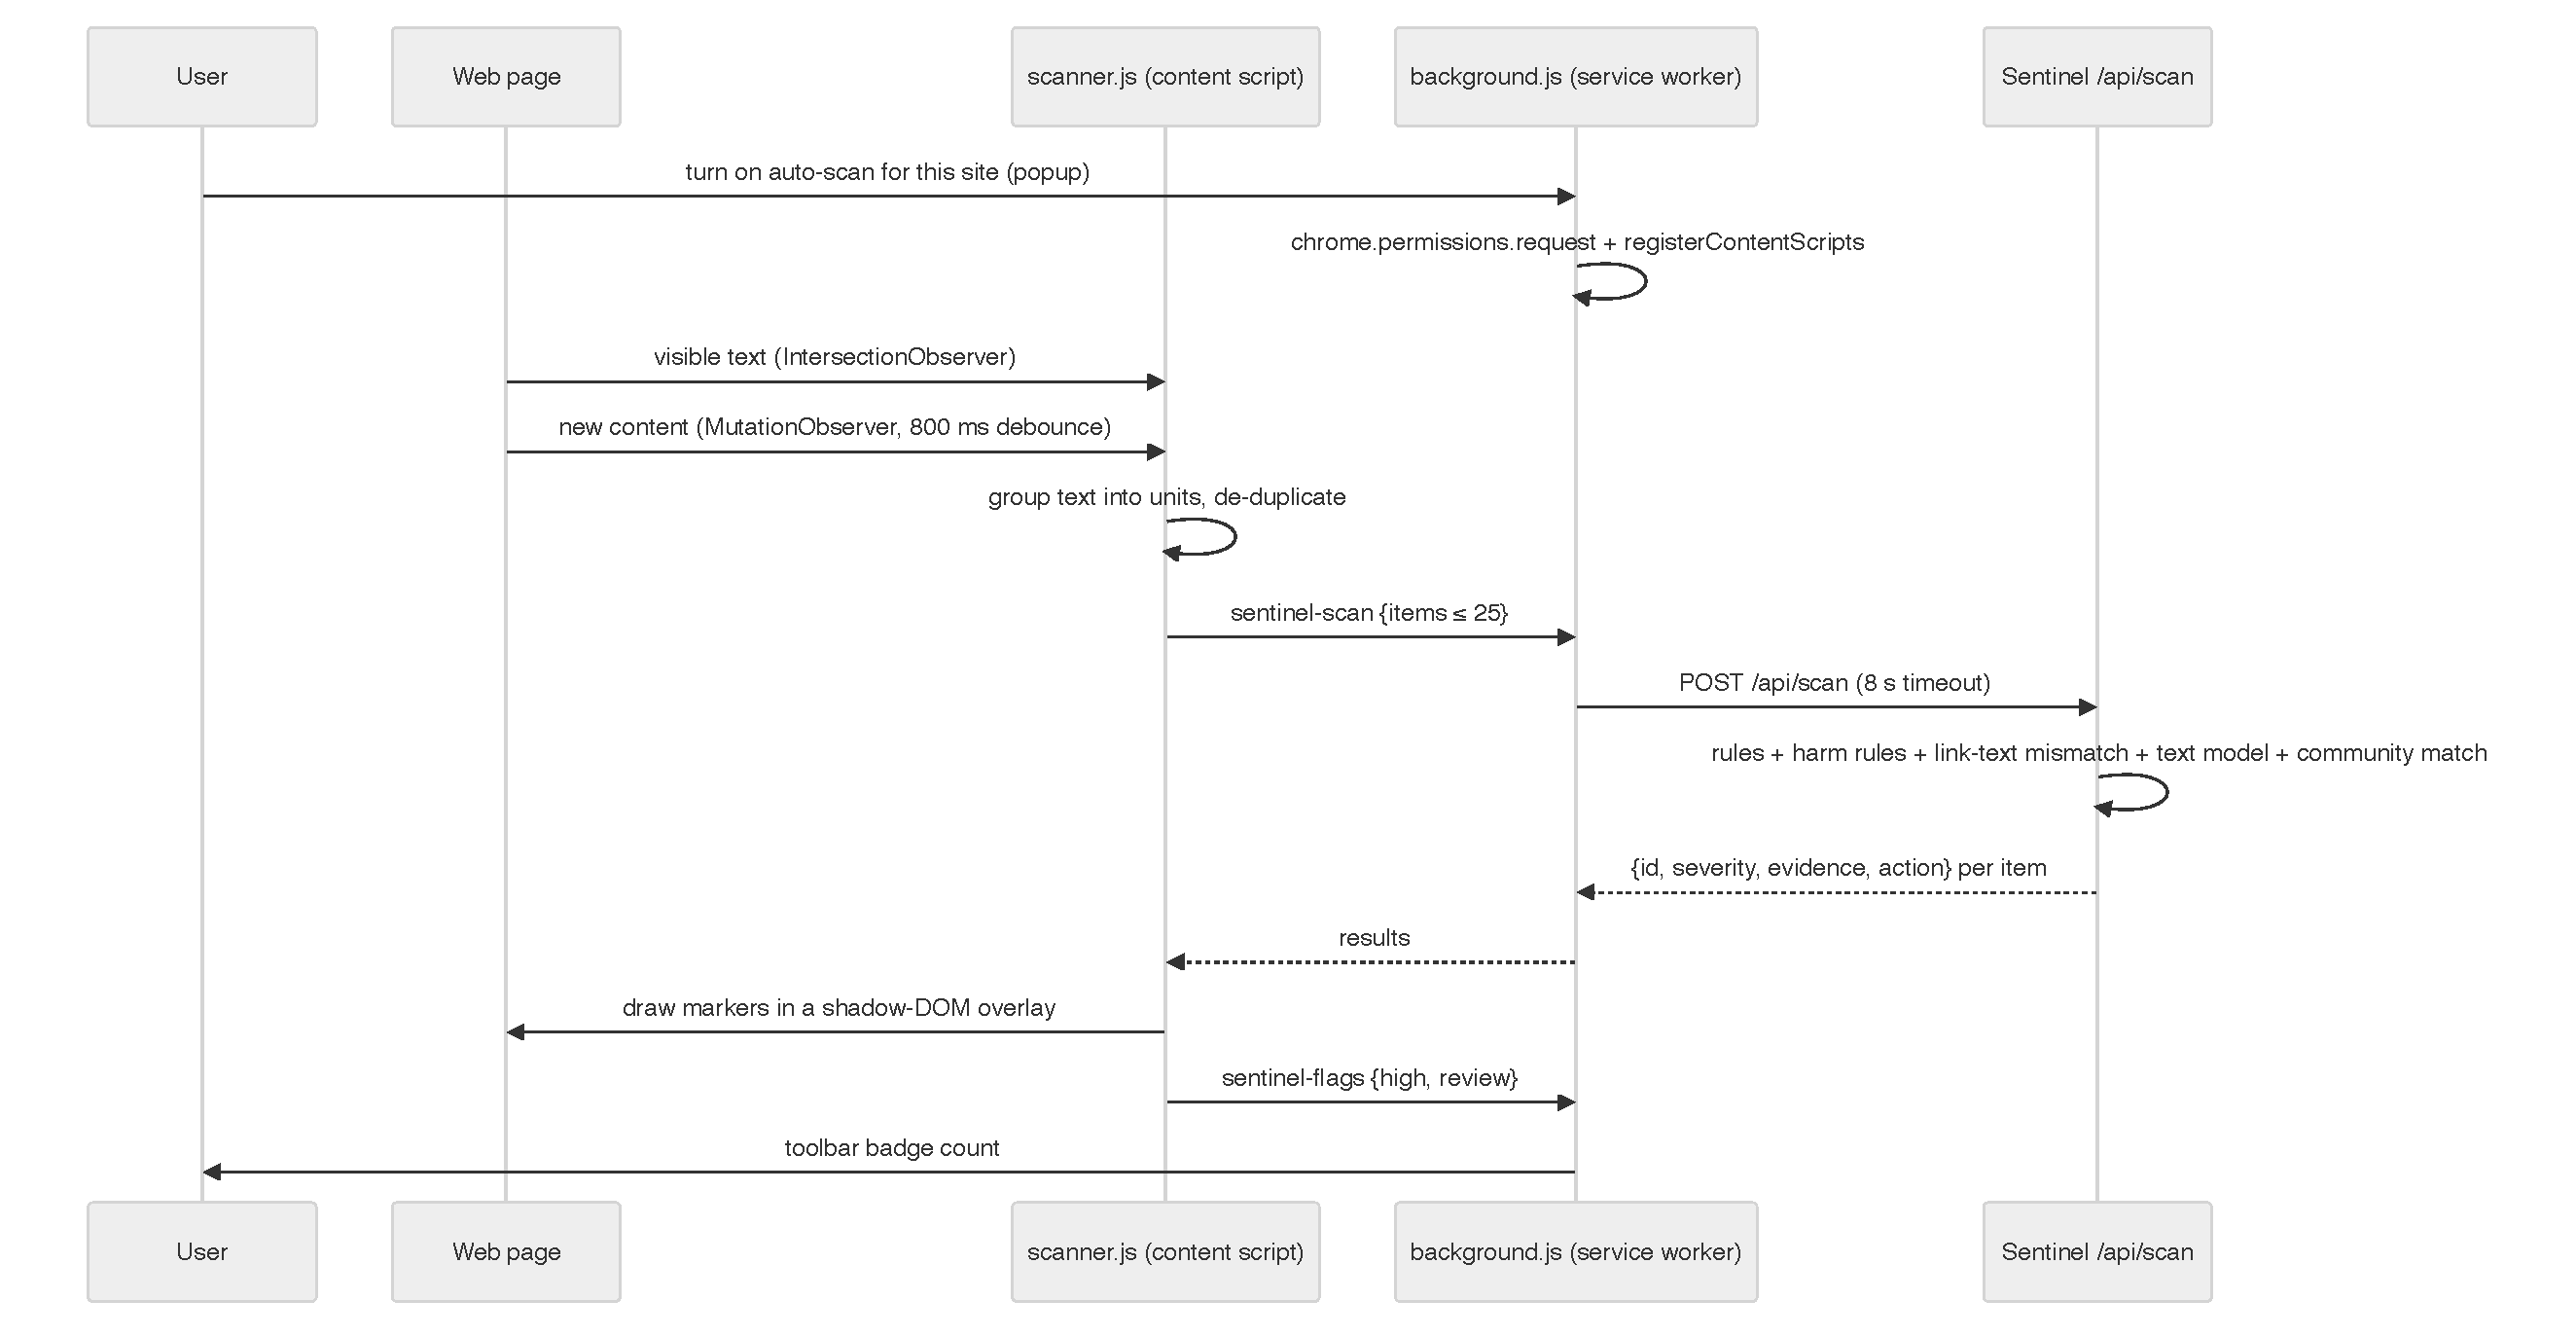
\includegraphics[width=0.92\linewidth]{dia2/autoscan.pdf}
\caption{Sequence Diagram: Auto-Scan}
\label{fig:autoscan}
\end{figure}
\begin{figure}[H]
\centering
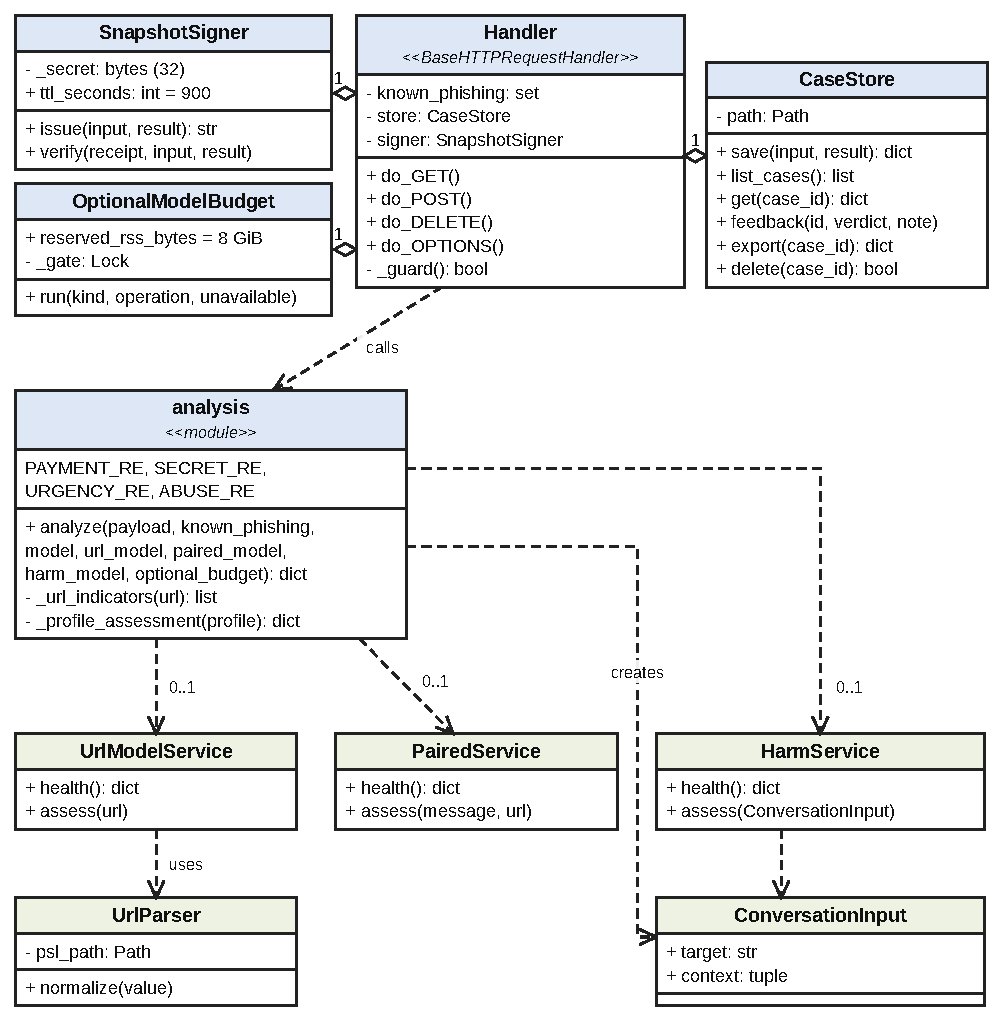
\includegraphics[width=0.78\linewidth]{dia/class.pdf}
\caption{Class Diagram}
\label{fig:class}
\end{figure}
\begin{figure}[H]
\centering
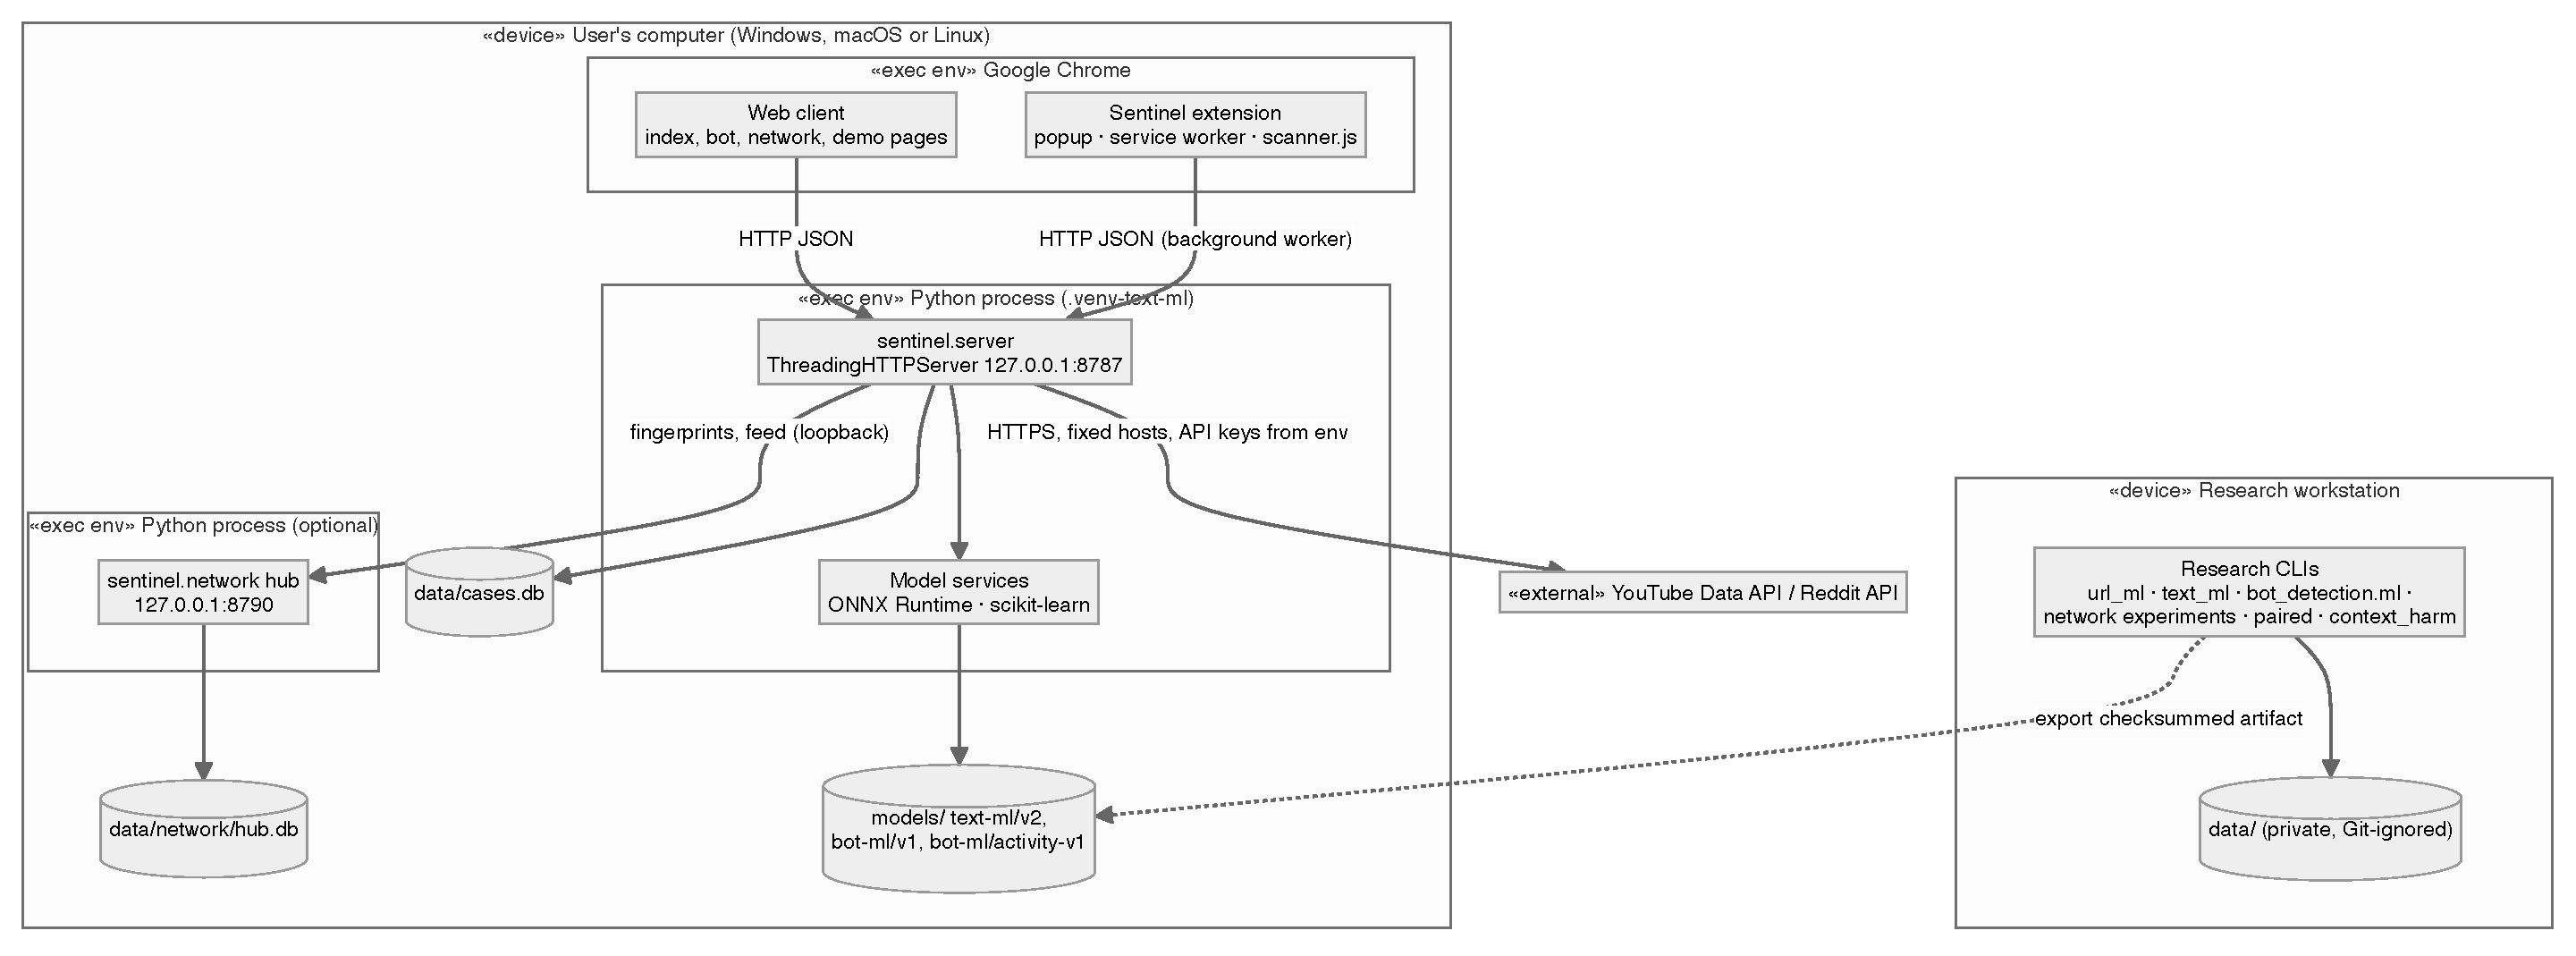
\includegraphics[width=\linewidth]{dia2/deploy_v2.pdf}
\caption{Deployment Diagram}
\label{fig:deploy}
\end{figure}

\subsection{ER-Diagram for the Database}
\noindent The ER diagram shows how saved cases are stored. Each case keeps the input, the exact result the user saw, the time and optional feedback. There are no user accounts. The optional community hub keeps its own database of fingerprints and report counts, with no message text.
\begin{figure}[H]
\centering
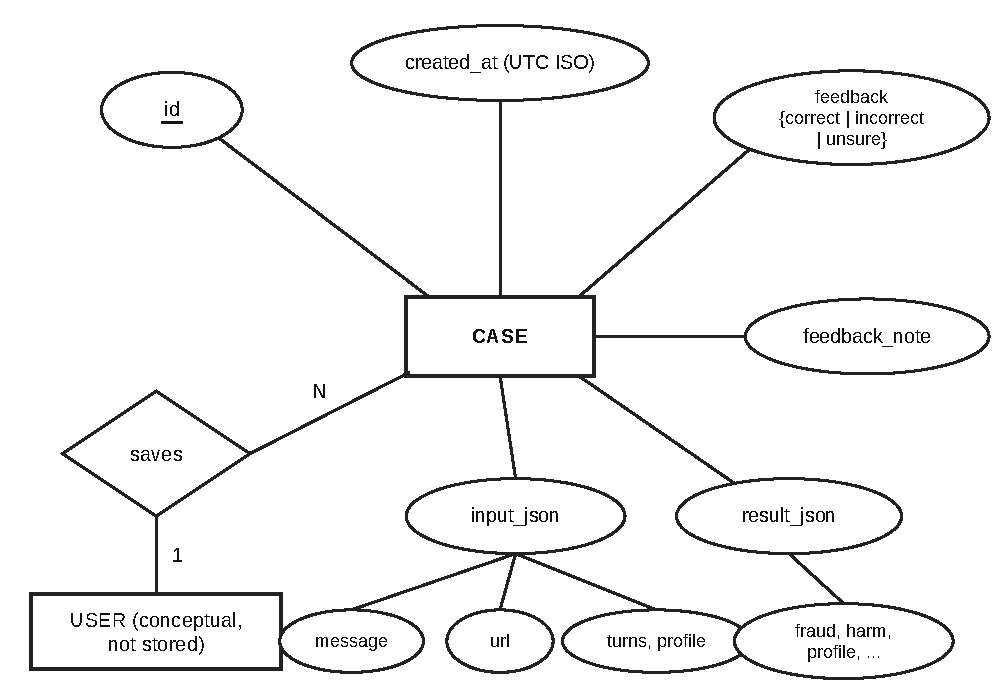
\includegraphics[width=0.62\linewidth]{dia/er.pdf}
\caption{ER Diagram}
\label{fig:er}
\end{figure}

\subsection{DFD (Min level 2)}
\noindent The data flow diagrams show how data moves from the user's input, through validation and the checkers, to the results and saved cases.
\begin{figure}[H]
\centering
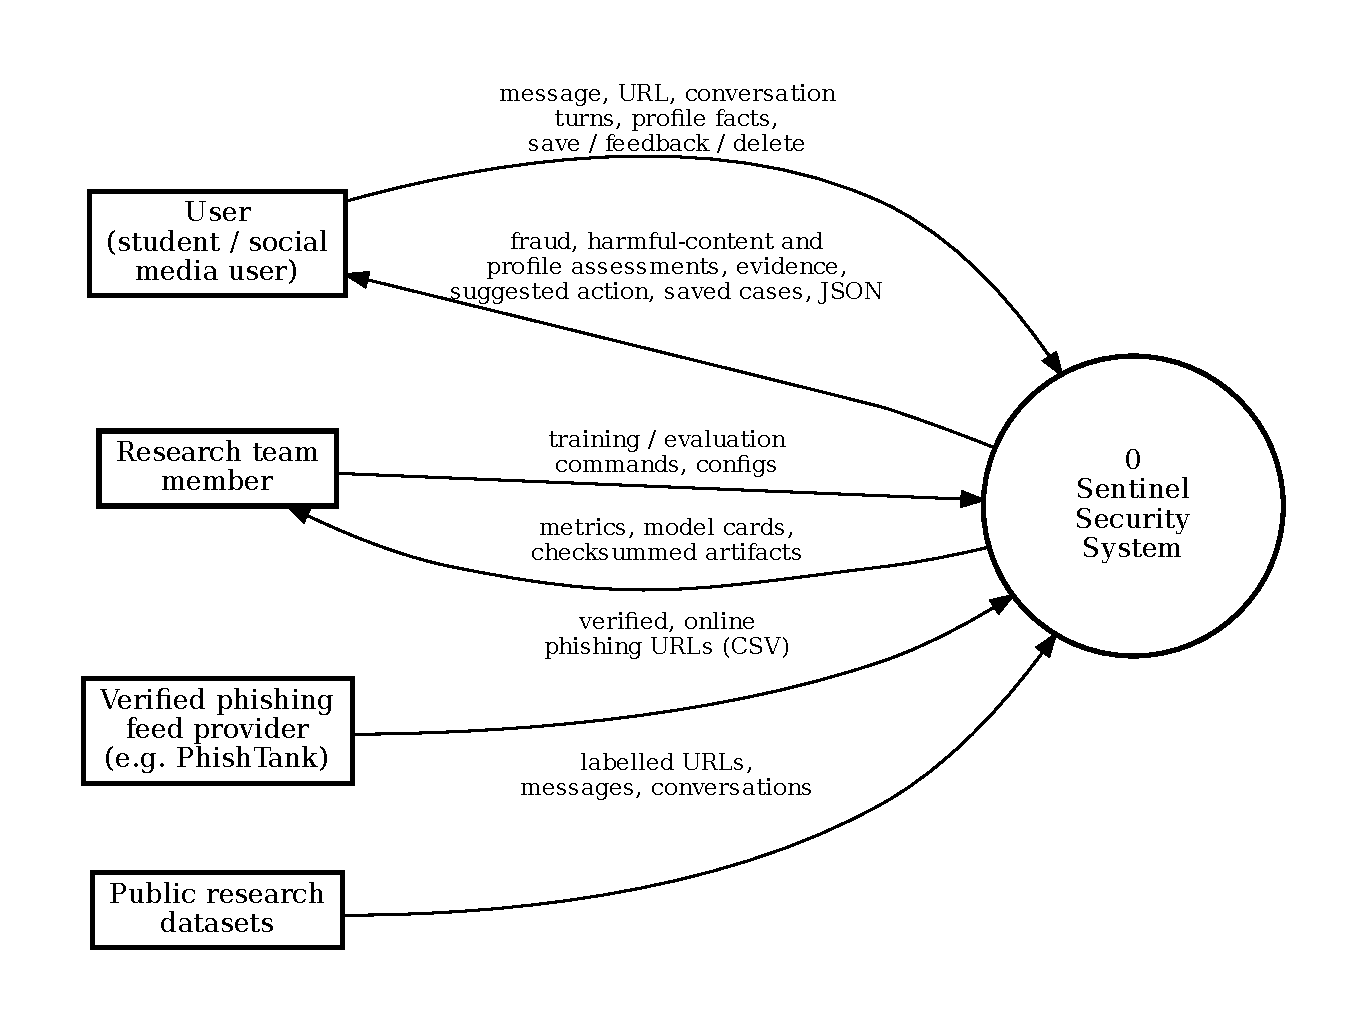
\includegraphics[width=0.7\linewidth]{dia/dfd0.pdf}
\caption{Data Flow Diagram: Level 0}
\label{fig:dfd0}
\end{figure}
\begin{figure}[H]
\centering
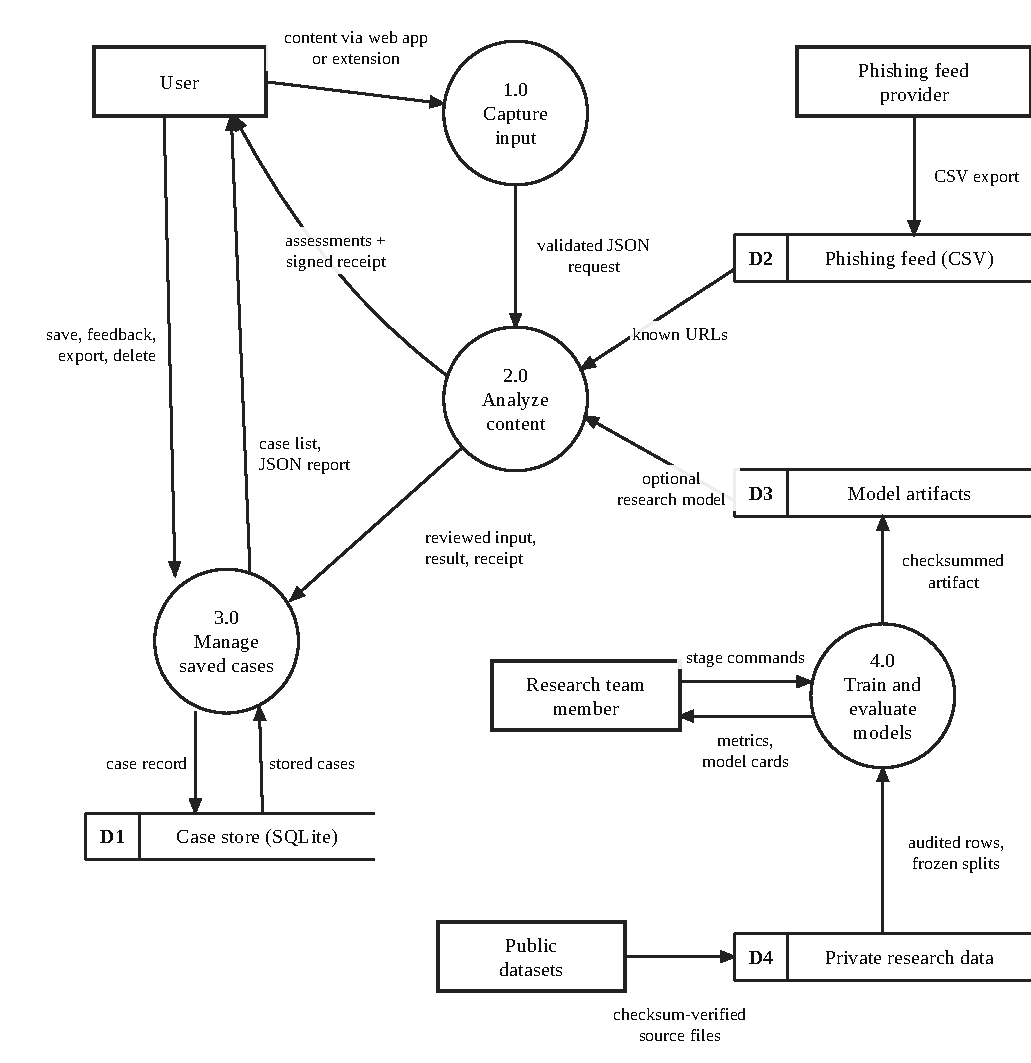
\includegraphics[width=0.78\linewidth]{dia/dfd1.pdf}
\caption{Data Flow Diagram: Level 1}
\label{fig:dfd1}
\end{figure}
\begin{figure}[H]
\centering
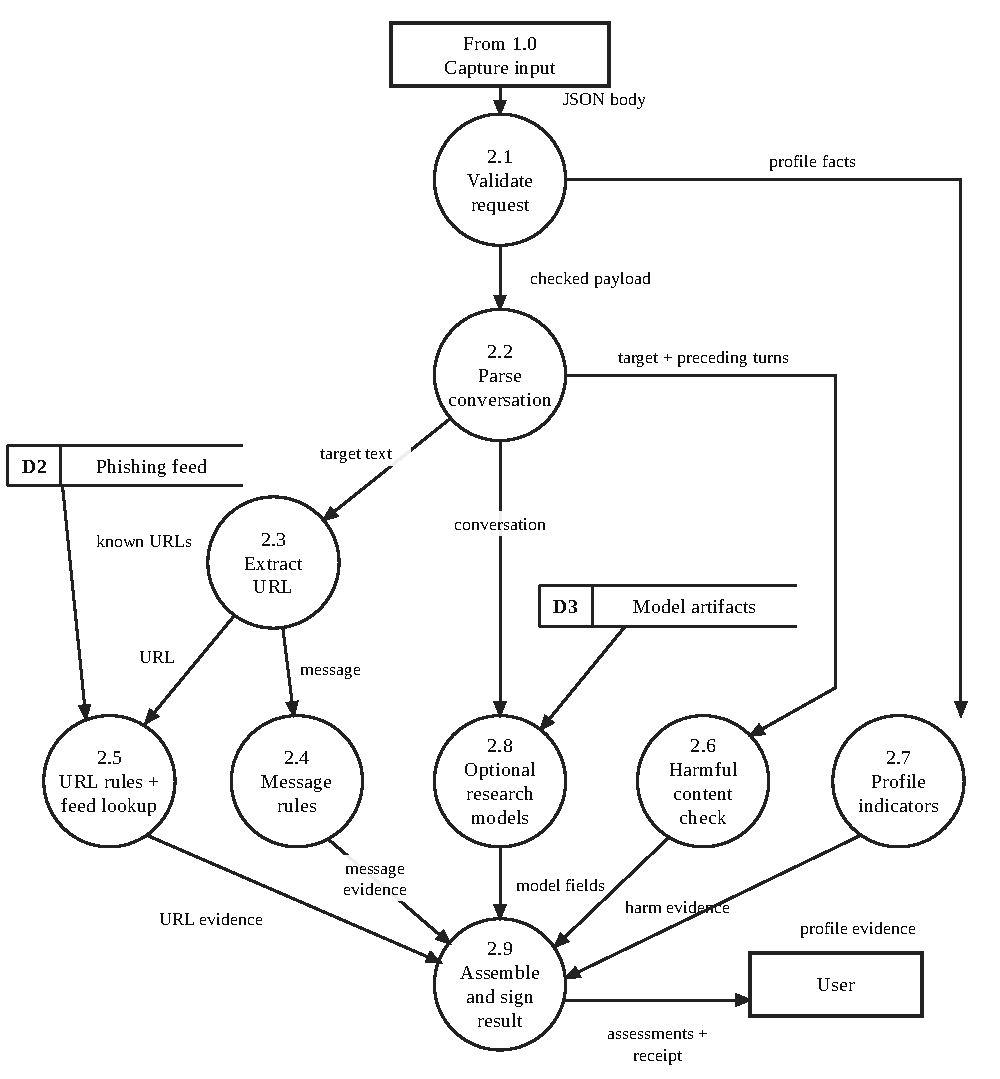
\includegraphics[width=0.78\linewidth]{dia/dfd2a.pdf}
\caption{Data Flow Diagram: Level 2 (Analyse Content)}
\label{fig:dfd2}
\end{figure}

\subsection{Algorithms / Methodology}
\noindent Sentinel combines clear rules with learned models. Each step is explained below.

\subsubsection*{1. Fraud Level}
\noindent If the link is on the known-phishing list, or the message asks for money or a password \emph{and} the link looks suspicious, the level is \textbf{High}. Any other evidence gives \textbf{Review}; otherwise \textbf{Low observed concern}.

\subsubsection*{2. Harmful-Language Check}
\noindent The text is cleaned of disguises, then each of the 19 rules is checked. Matches inside known idioms are skipped. A negation just before a match (``never'', ``not'') lowers the level, and quoted or reported text is lowered from High to Review, except for self-harm risk. The final level is the highest one found, and the advice comes from the most urgent category.

\subsubsection*{3. Scam-Text Model}
\noindent DistilBERT's scores $\mathbf{z}$ are calibrated with a temperature $T=1.29$ and averaged with the TF-IDF model's probabilities $\mathbf{p}^{\mathrm{L}}$:
\begin{equation}
\mathbf{p}=\tfrac12\big(\mathrm{softmax}(\mathbf{z}/T)+\mathbf{p}^{\mathrm{L}}\big),\qquad s=p_{\mathrm{spam}}+p_{\mathrm{smishing}}
\end{equation}
A warning is shown when $s\ge0.611$. This threshold was chosen on separate data so that at most 1\% of genuine messages are flagged. To explain a warning, each word is removed in turn and the drop in the score is measured.

\subsubsection*{4. Community Fingerprints}
\noindent A message is cut into 3-word pieces and 64 hash functions give a MinHash fingerprint \cite{broder}. Two messages with similarity $J$ share at least one of 32 fingerprint ``bands'' with probability
\begin{equation}
P(J)=1-\big(1-J^{2}\big)^{32}
\end{equation}
which is 99.7\% at $J=0.41$, so reworded scams still match \cite{mmds}. A scam is published only after 5 different reporters ($k$-anonymity \cite{sweeney}).
\begin{figure}[H]
\centering
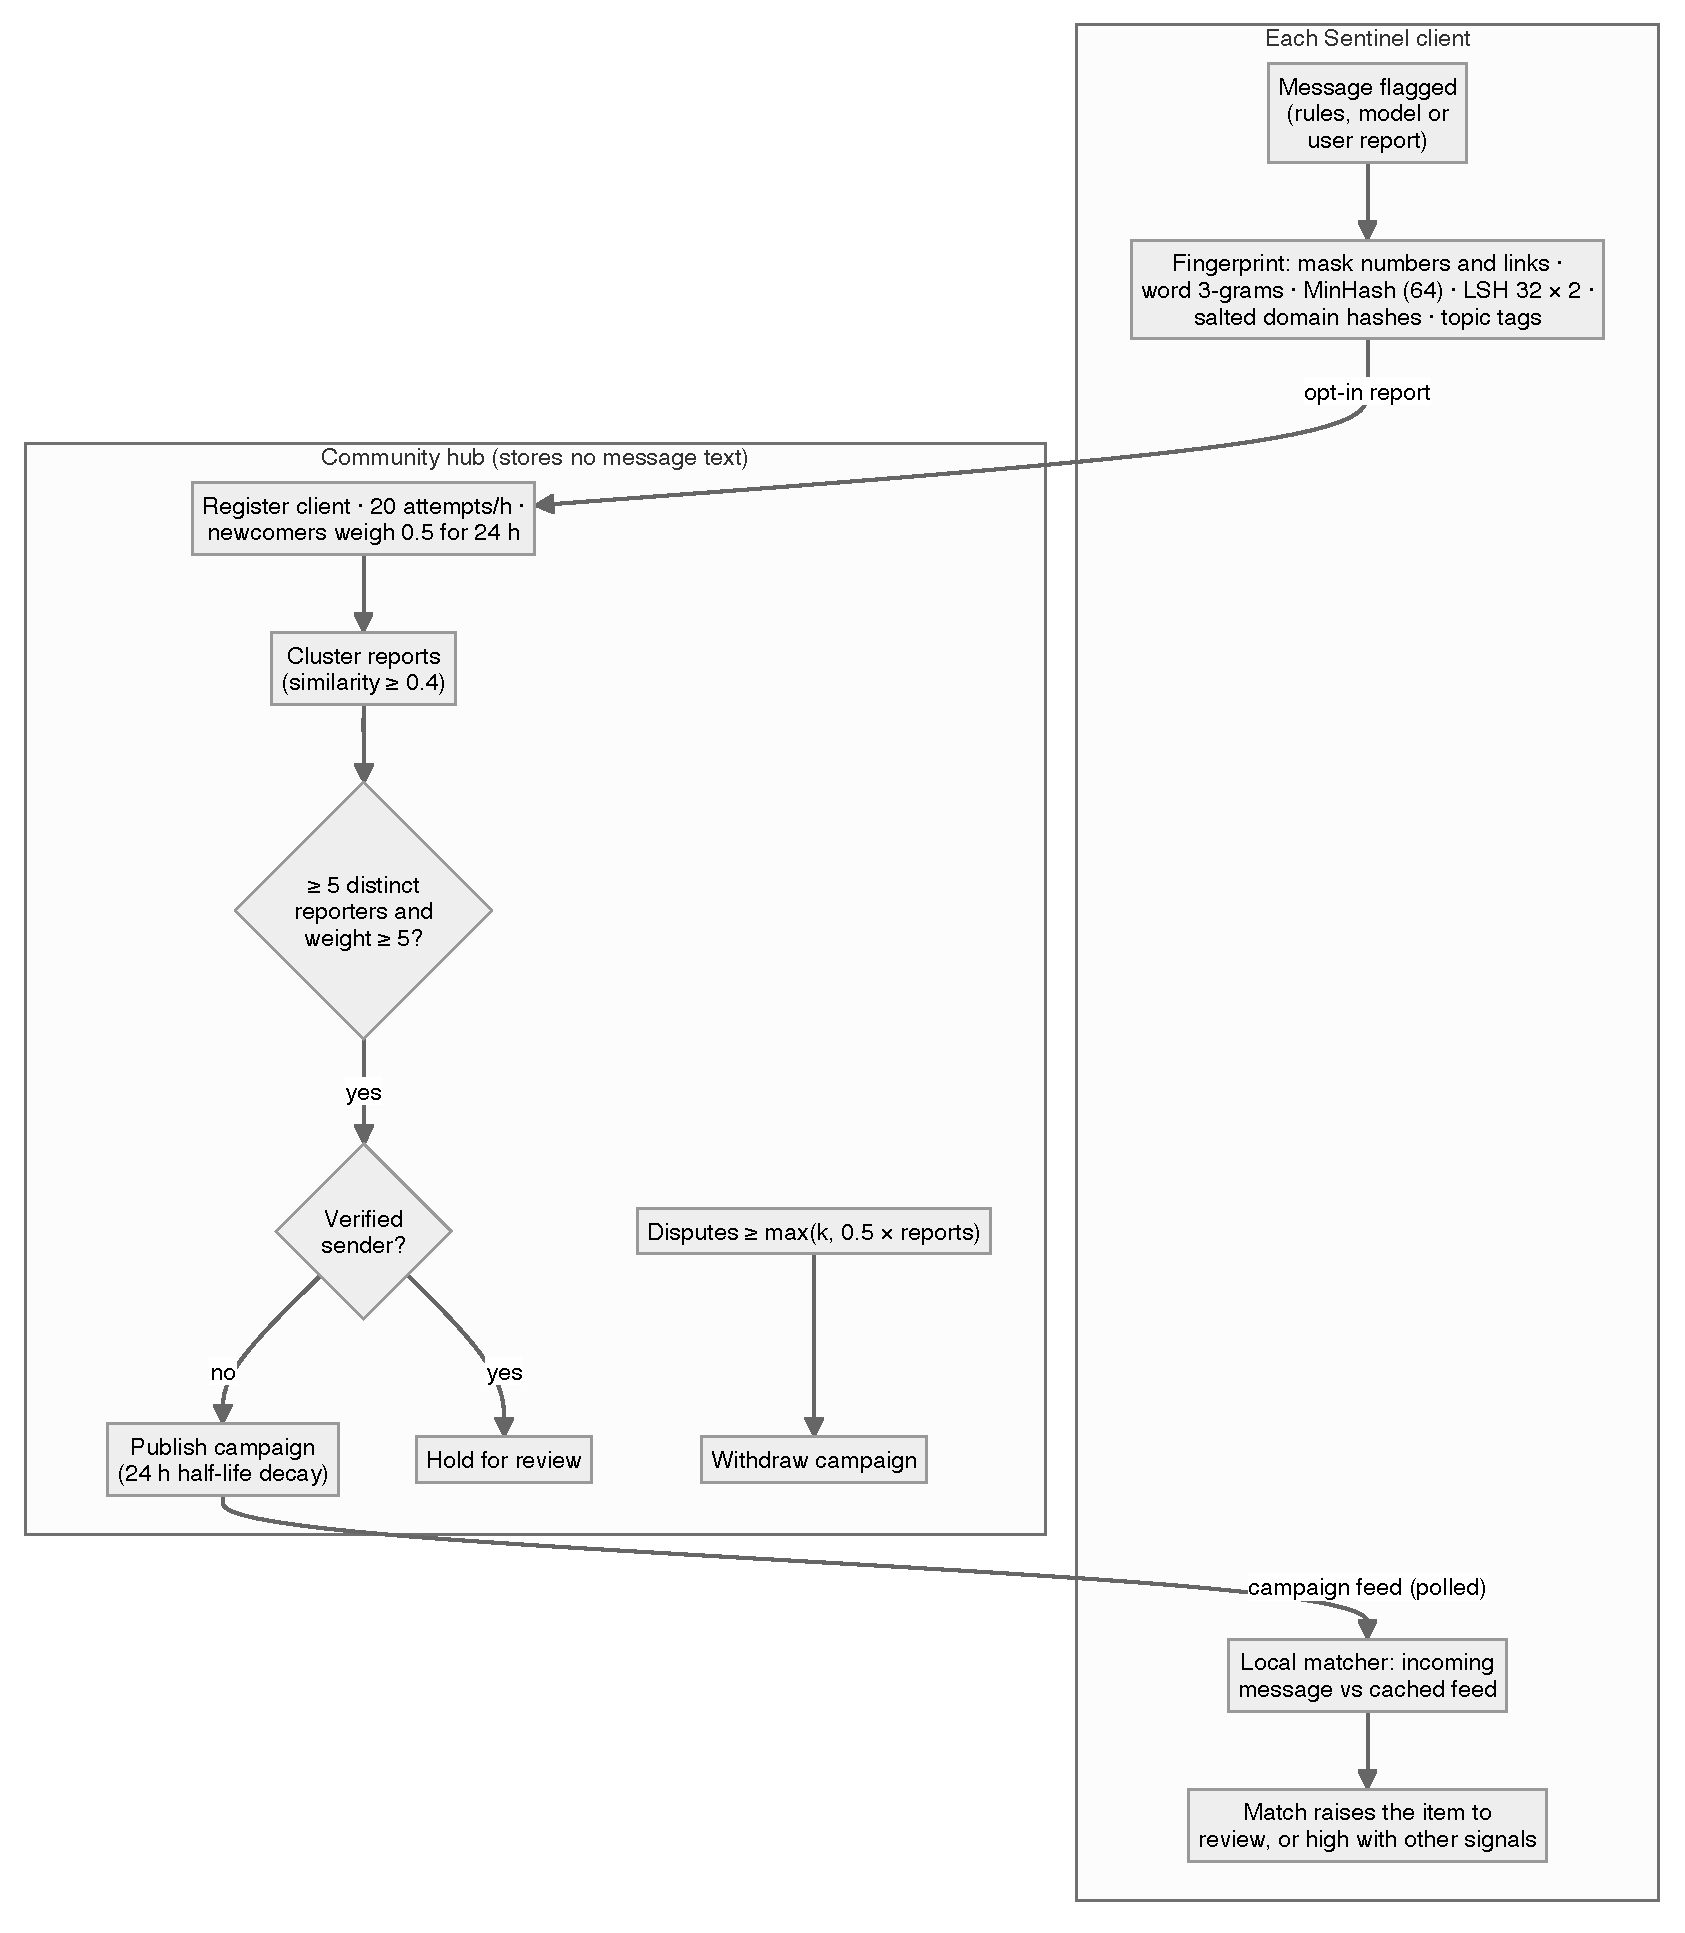
\includegraphics[width=0.5\linewidth]{dia2/network.pdf}
\caption{Community Scam Network}
\label{fig:network}
\end{figure}

\subsubsection*{5. Bot Score}
\noindent Each of the 25 signals gives a suspicion $s_i$ between 0 and 1 and has a weight $w_i$. Only signals with data ($A$) are used:
\begin{equation}
\text{score}=100\cdot\frac{\sum_{i\in A} w_i s_i}{\sum_{i\in A} w_i}
\end{equation}
If too little data is available, the score is not shown. The trained models use gradient boosting \cite{sklearn} with calibrated probabilities \cite{zadrozny}, and are used only if they reach an AUC of at least 0.80 on every dataset they were not trained on \cite{yang2020}.
\begin{figure}[H]
\centering
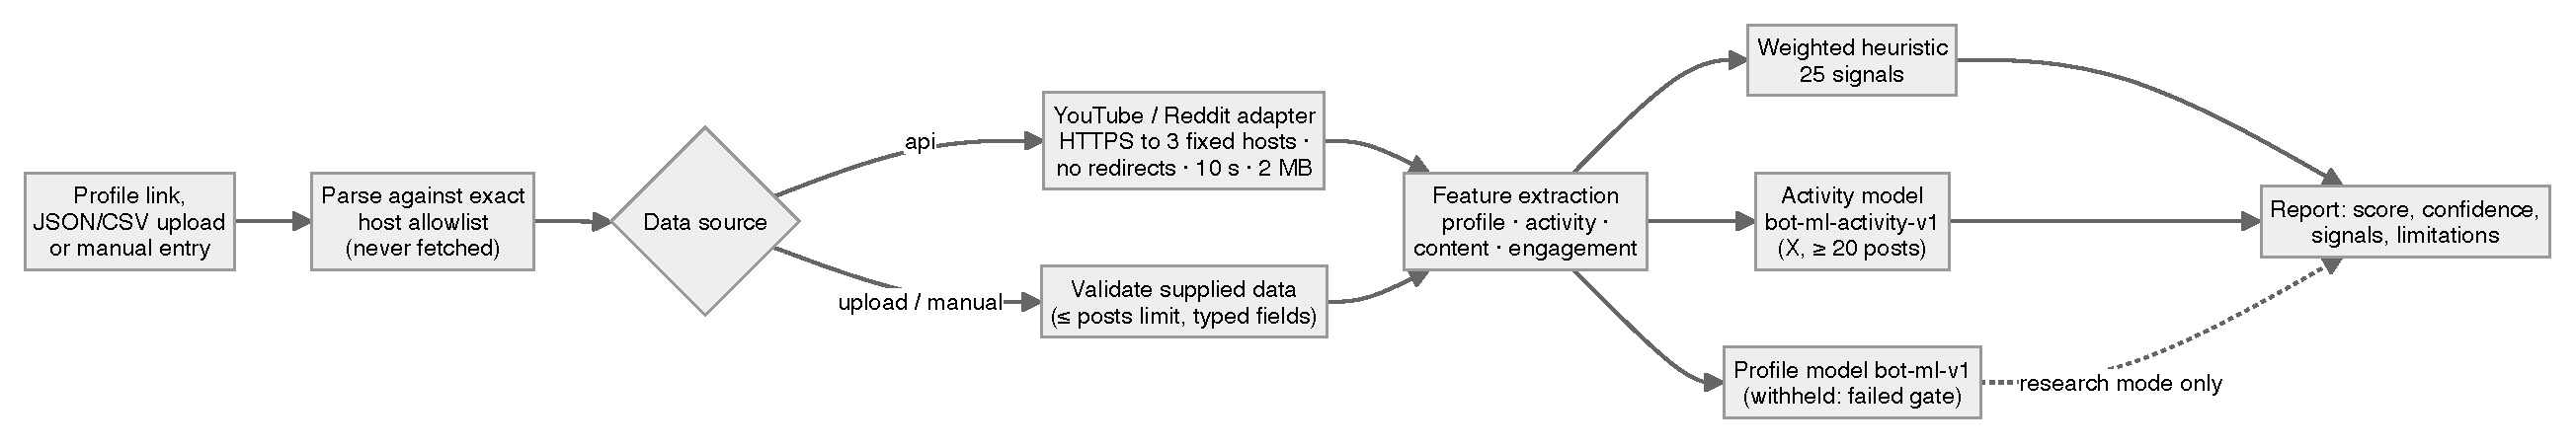
\includegraphics[width=\linewidth]{dia2/bot.pdf}
\caption{Bot Detection Pipeline}
\label{fig:bot}
\end{figure}

\subsubsection*{Overall Algorithm}
\begin{enumerate}
\item Start the Sentinel server and open the web app or extension.
\item Receive a message, link, chat or account, or scan the visible page.
\item Validate the request and read links as text only.
\item Run fraud rules, harm rules, the scam-text model and community matching.
\item For accounts, score the 25 signals and add the trained model's probability where allowed.
\item Build a separate result for each threat with evidence, missing checks and a next step.
\item Show the results as cards or page markers.
\item Save the case if the user asks, after checking its receipt.
\item With auto-scan on, repeat for every new message on the page.
\end{enumerate}

\subsection{UI/UX Design}
\noindent The interface is simple and honest: plain language, separate results for each threat, a text label on every level (not just colour), and nothing stored unless the user chooses.

\noindent\textbf{1. Check Content Screen}\\
The input is on the left and the result cards on the right. Each card shows the level, the evidence, what could not be checked and a next step. The learned-model card underlines the words that raised the scam score.
\begin{figure}[H]
\centering
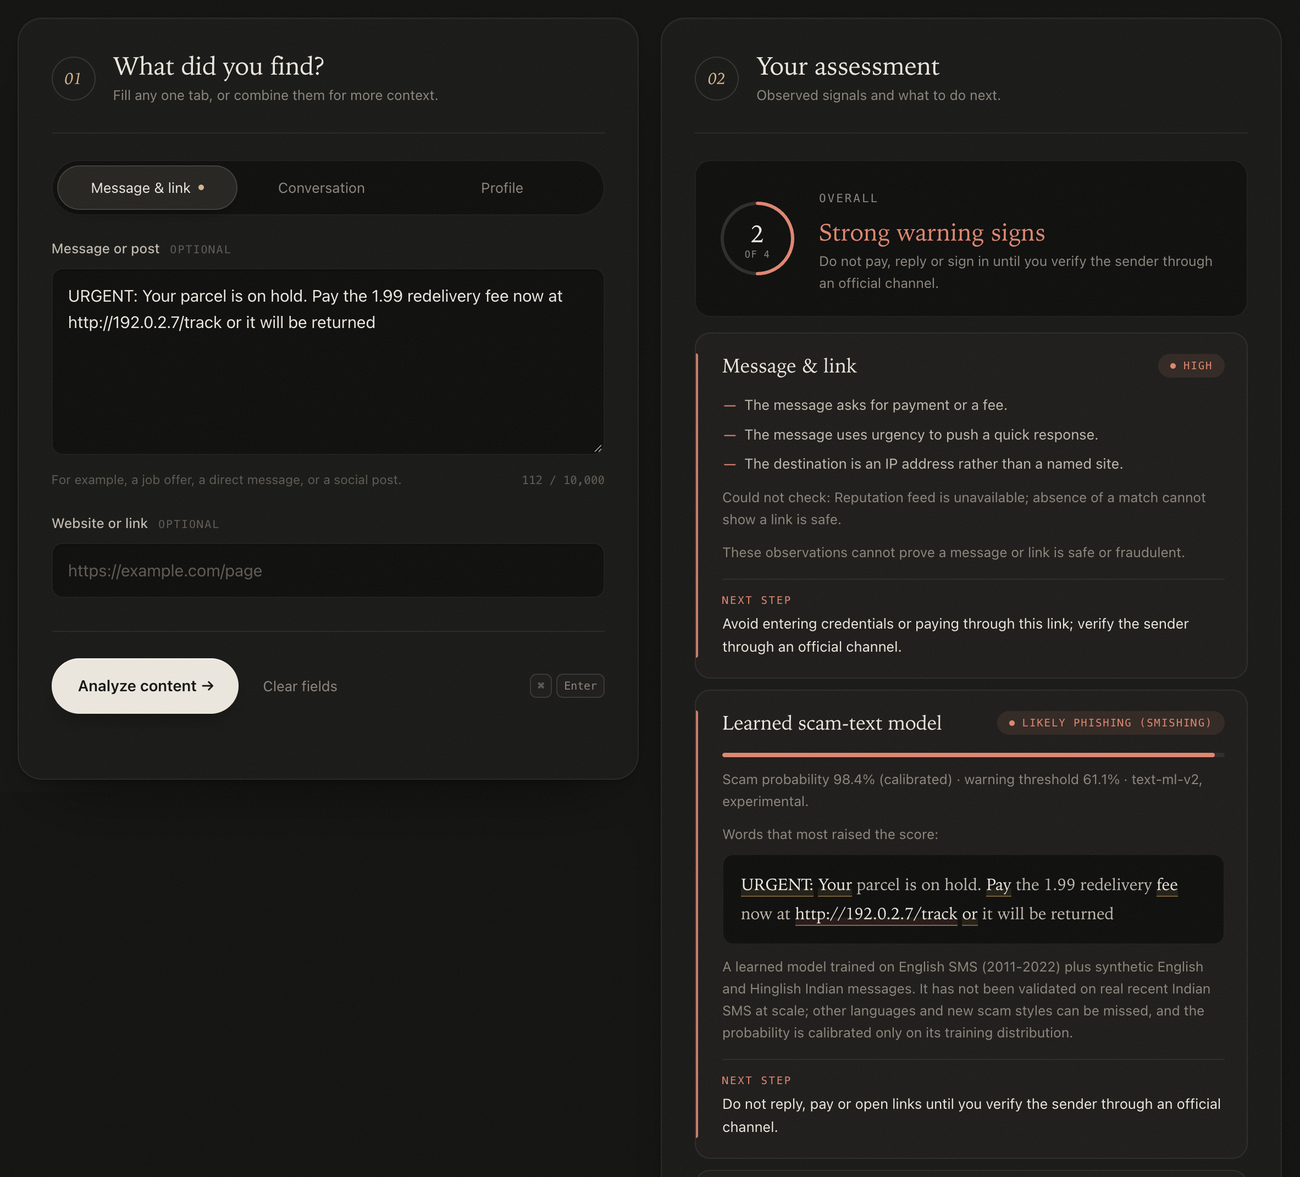
\includegraphics[width=0.85\linewidth]{shots2/check_scam.png}
\caption{Sentinel Check Content Screen}
\label{fig:ui-check}
\end{figure}

\noindent\textbf{2. Harmful-Language Result}\\
When a message is a threat, the harmful-content card moves to the top with clear advice.
\begin{figure}[H]
\centering
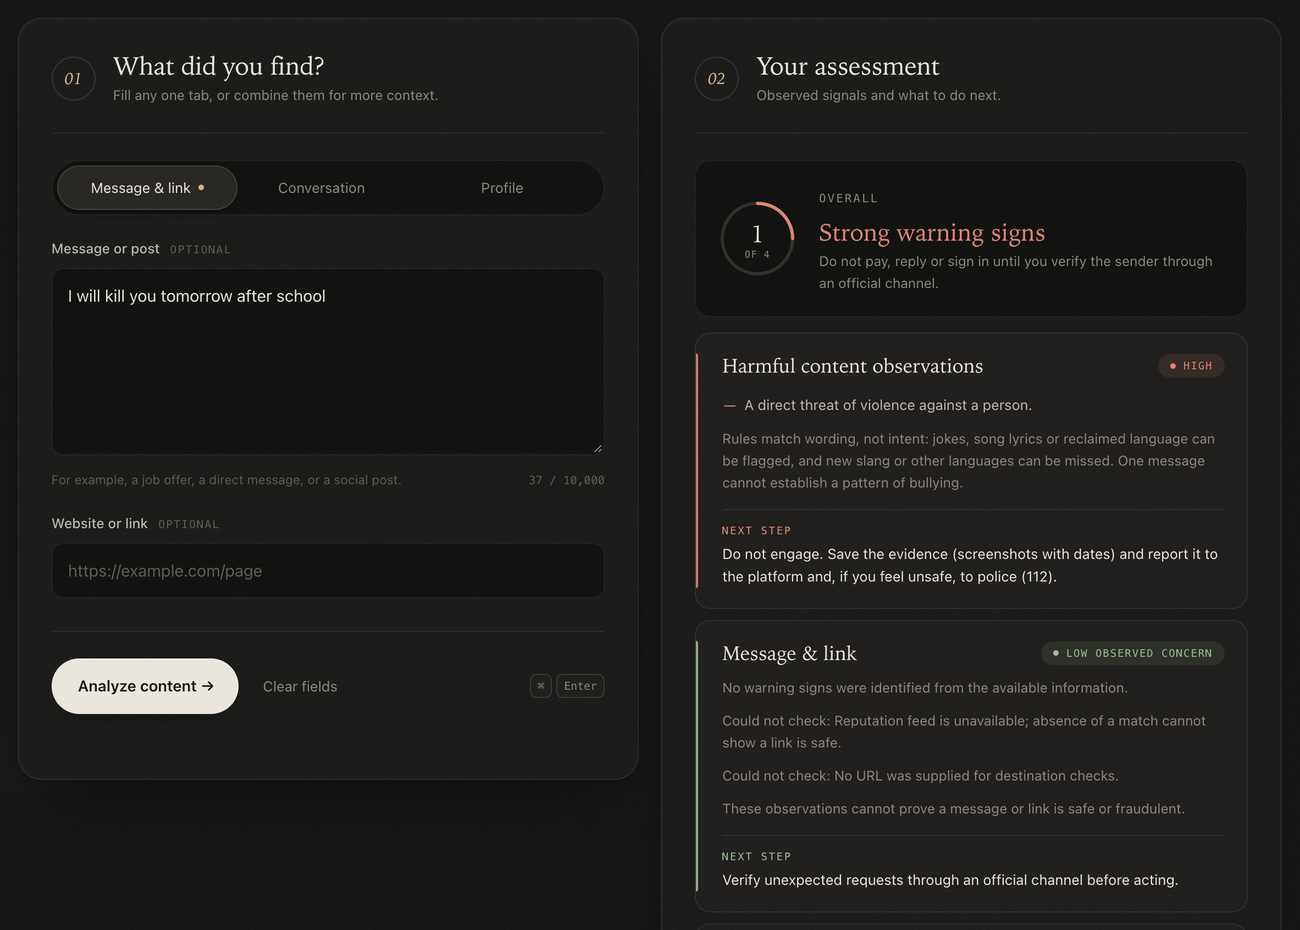
\includegraphics[width=0.85\linewidth]{shots2/check_threat.png}
\caption{Sentinel Harmful-Language Result}
\label{fig:ui-threat}
\end{figure}

\noindent\textbf{3. Bot Accounts Screen}\\
A gauge shows the bot score, with the confidence, data coverage and the signals behind the score.
\begin{figure}[H]
\centering
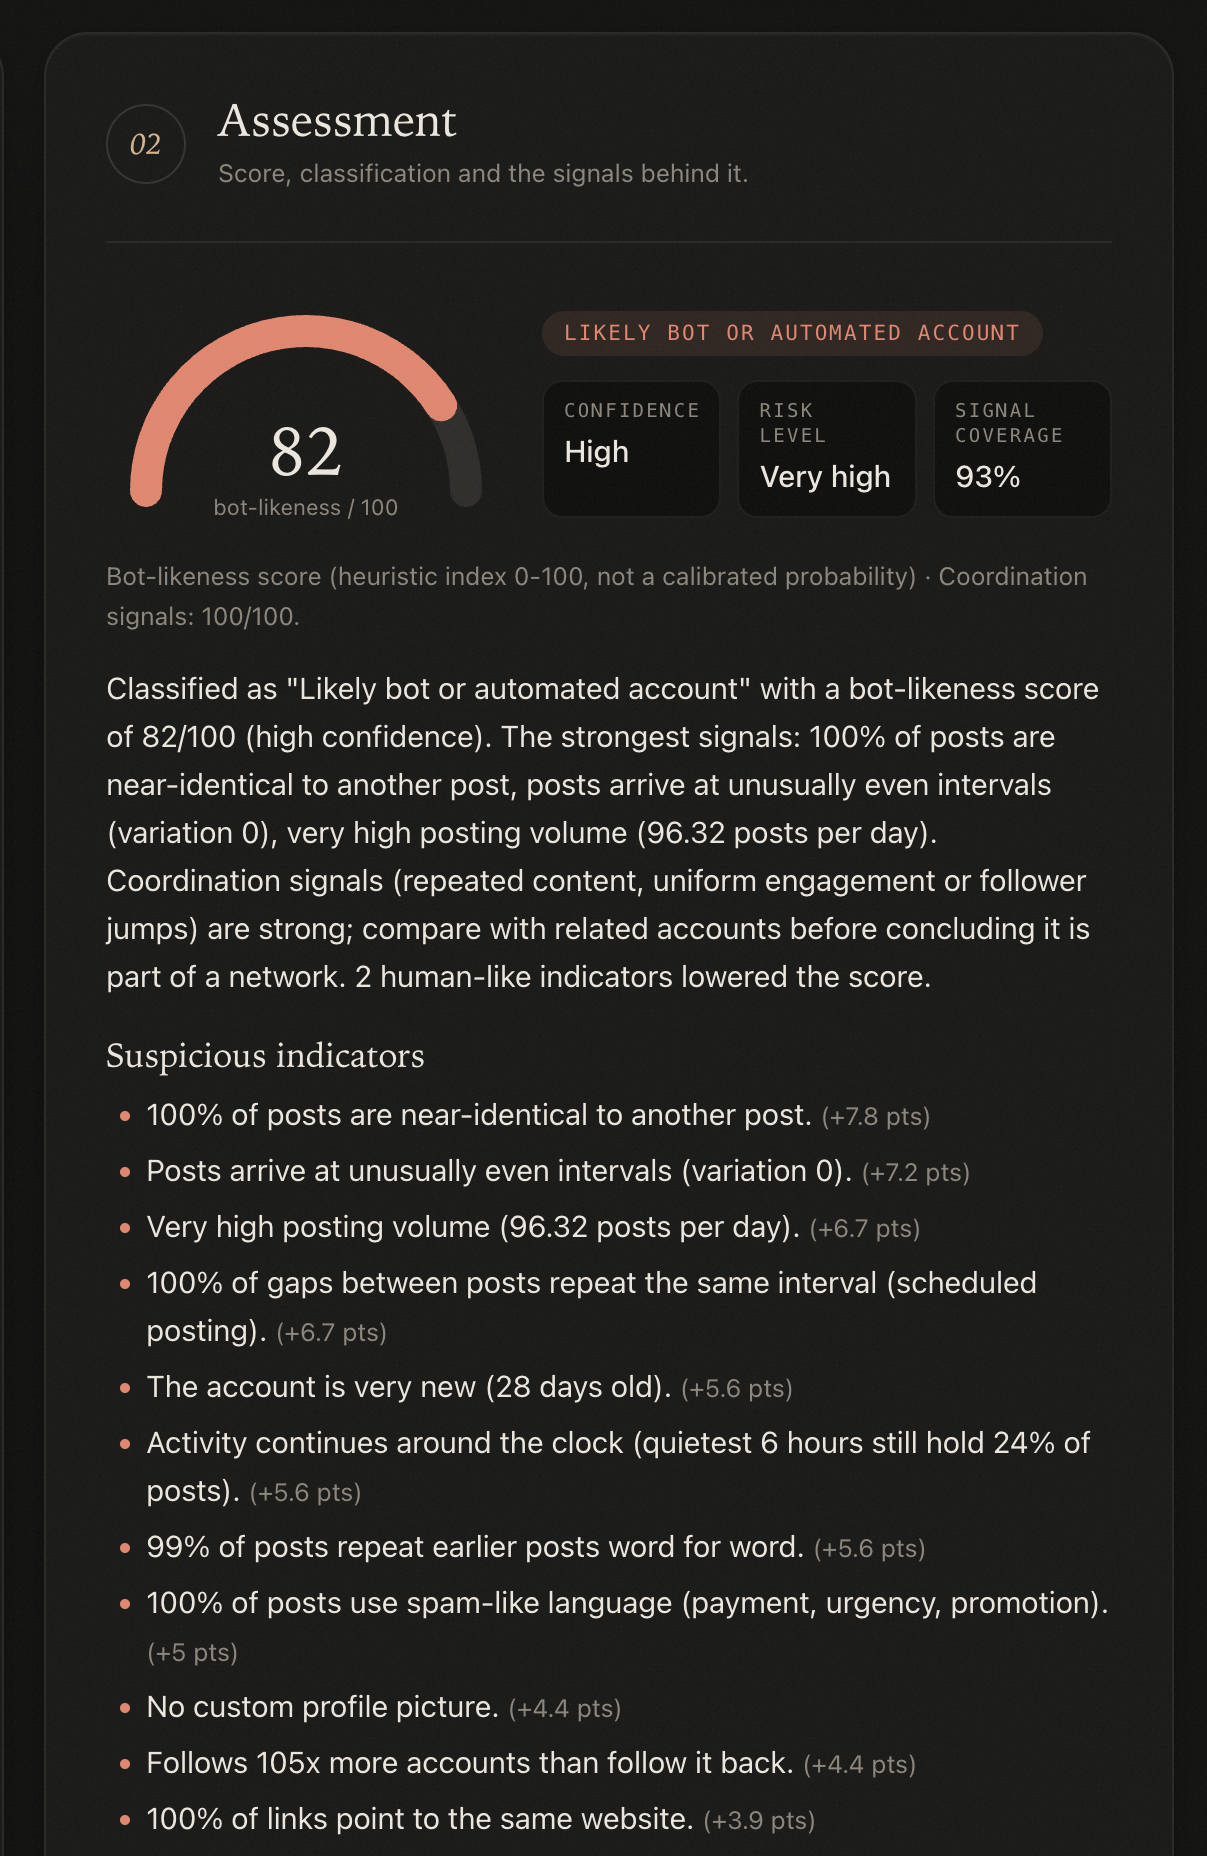
\includegraphics[width=0.48\linewidth]{shots2/bot_report_panel.png}
\caption{Sentinel Bot Accounts Screen}
\label{fig:ui-bot}
\end{figure}

\noindent\textbf{4. Community Network Screen}\\
This page shows the live scam campaigns published by the hub and explains what the hub stores.
\begin{figure}[H]
\centering
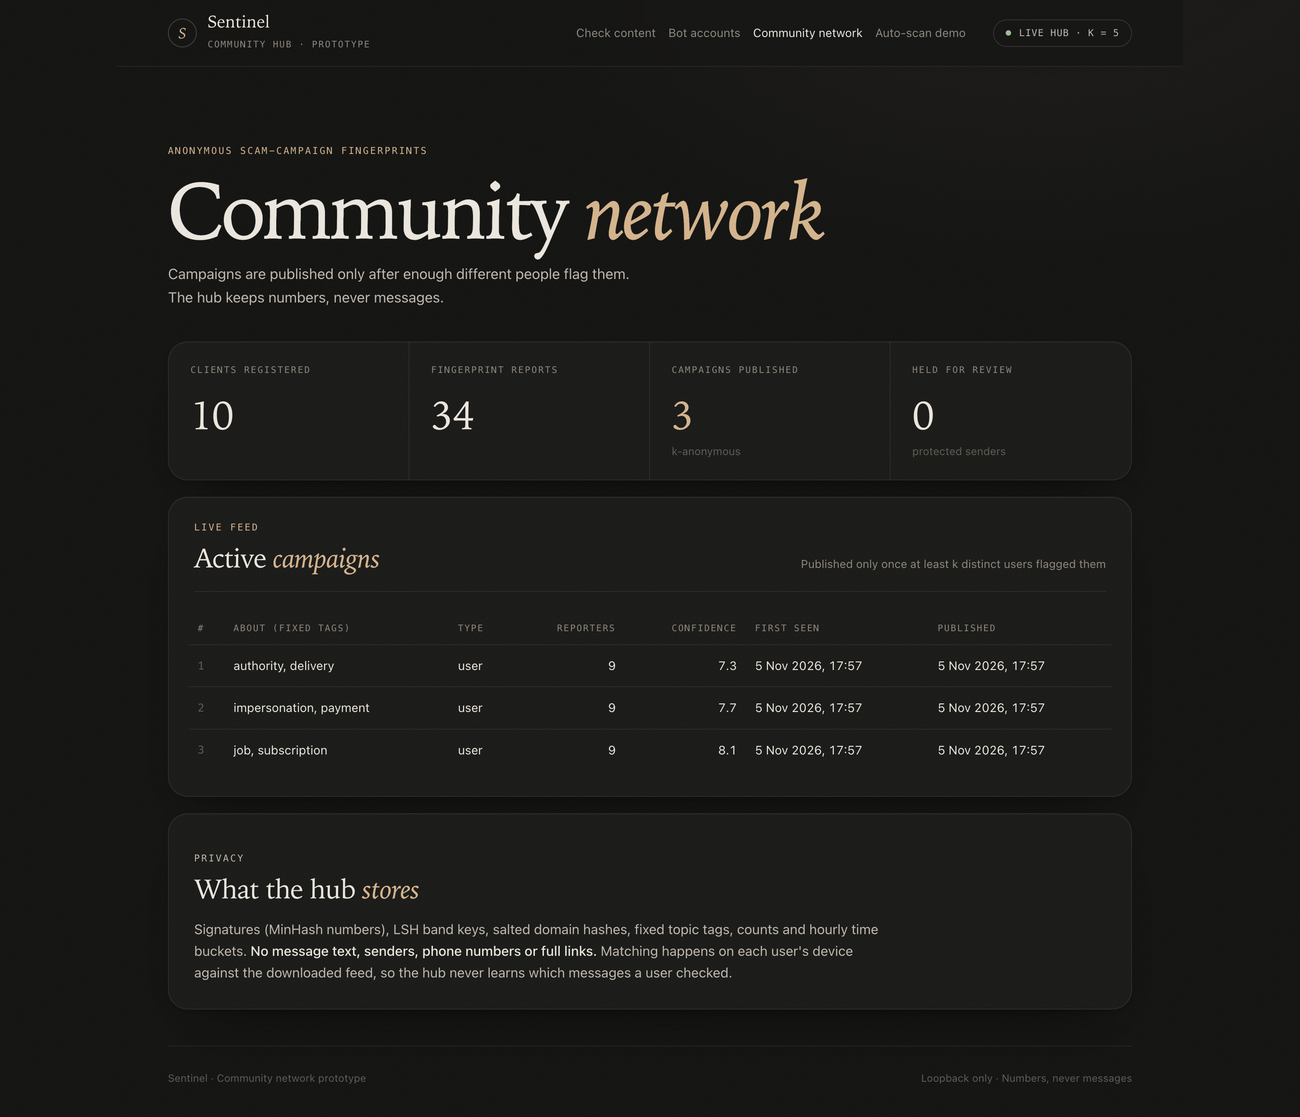
\includegraphics[width=0.85\linewidth]{shots2/network.png}
\caption{Sentinel Community Network Screen}
\label{fig:ui-network}
\end{figure}

\noindent\textbf{5. Auto-Scan Demo and Extension Popup}\\
The demo chat page is used to show auto-scan marking scam messages as they arrive. The popup offers quick checks and the auto-scan switch (the popup screenshot is older than the switch).
\begin{figure}[H]
\centering
\begin{minipage}[b]{0.64\linewidth}\centering
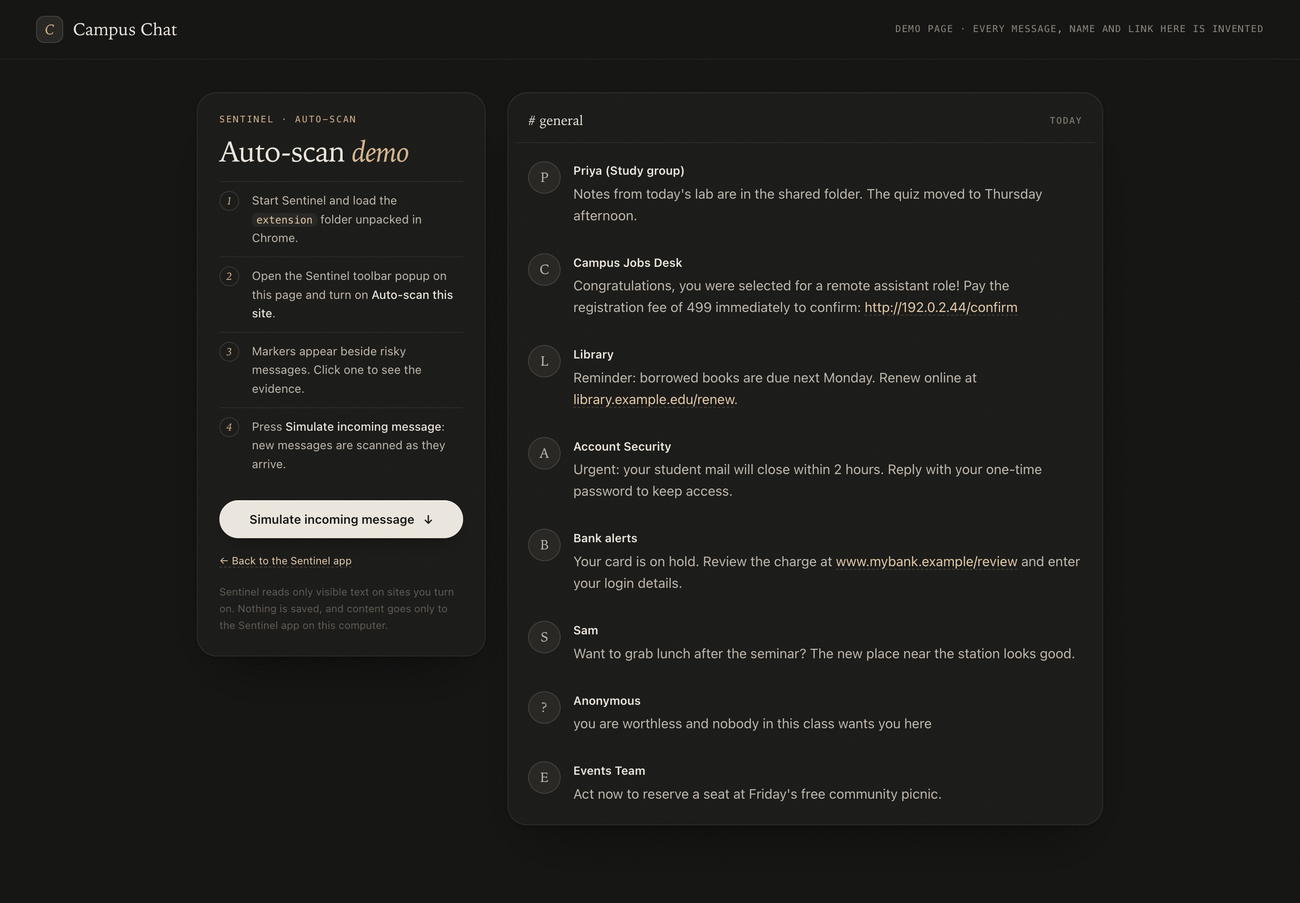
\includegraphics[width=\linewidth]{shots2/demo.png}\\[1pt]{\small (a) Auto-scan demo chat page}
\end{minipage}\hfill
\begin{minipage}[b]{0.3\linewidth}\centering
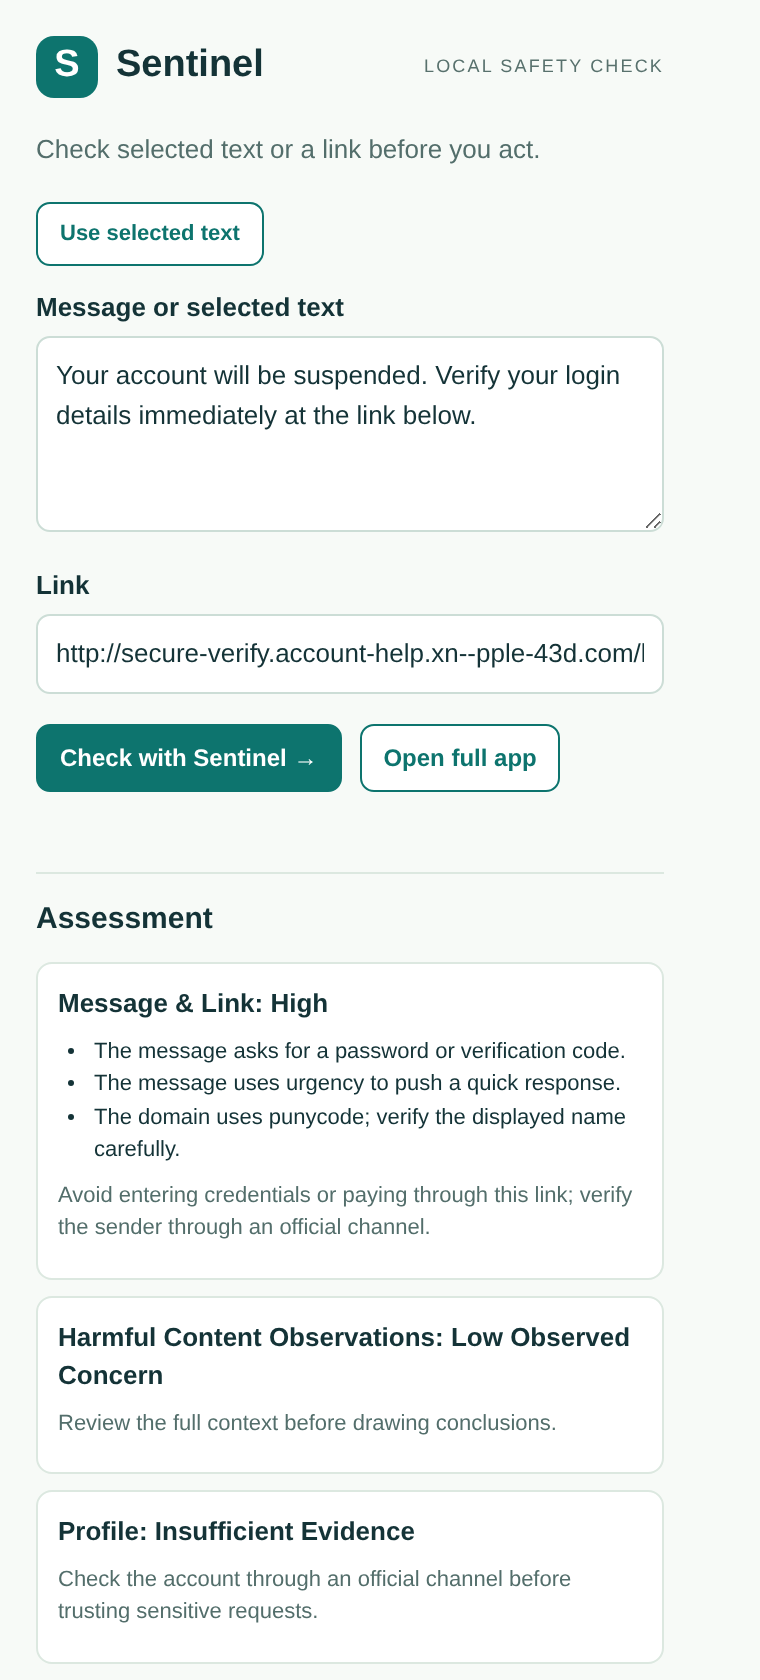
\includegraphics[width=\linewidth]{shots/13_popup_crop.png}\\[1pt]{\small (b) Extension popup}
\end{minipage}
\caption{Sentinel Auto-Scan Demo Page and Extension Popup}
\label{fig:ui-ext}
\end{figure}

\noindent Overall, the design gives clear access to checking content, checking accounts and seeing community warnings, and helps users understand why each result was given.
